\documentclass[11pt]{article}

% Mode is controlled by the `acl-mode` YAML field:
%   review   — anonymous, line numbers (default for submission)
%   final    — camera-ready, authors shown
%   preprint — non-anonymous, page numbers
% acl.sty handles: geometry (a4, 2.5cm margins), twocolumn, natbib,
%   caption, hyperref, bibliographystyle{acl_natbib}.
% Do NOT load those packages again here.
\usepackage[review]{acl}

% Packages from the official ACL template (acl_latex.tex) — safe to load after acl.sty
\usepackage{times}
\usepackage{latexsym}
\usepackage[T1]{fontenc}
\usepackage[utf8]{inputenc}
\usepackage{textcomp}   % euro sign and other symbols
\usepackage{microtype}
\usepackage{inconsolata}

% Math
\usepackage{amsmath}
\usepackage{amssymb}

% Tables — all three needed for pandoc's longtable output
\usepackage{longtable}
\usepackage{booktabs}
\usepackage{array}     % pandoc uses >{\raggedright\arraybackslash}p{} column types
\usepackage{calc}      % pandoc uses \real{} expressions for column widths
\usepackage{multirow}  % multi-row table cells

\usepackage{etoolbox}

% longtable is incompatible with twocolumn mode (enforced by acl.sty), which is
% why this file used to wrap every longtable in \onecolumn ... \twocolumn:
%
%   \BeforeBeginEnvironment{longtable}{\onecolumn}
%   \AfterEndEnvironment{longtable}{\twocolumn}
%
% Every table in this paper now lives in the appendix, which is already
% \onecolumn. Under those hooks the trailing \twocolumn would flip the appendix
% into two columns after the first table, and each switch forces a page break.
% They are removed deliberately. Restore them only if a longtable is ever
% needed in the two-column main text.

% Fix table caption numbering for longtable
\def\fnum@table{\tablename~\thetable}

% Float placement. Main-text floats use LaTeX's default [tbp] so they can move
% to wherever they fit, including across section boundaries; pinning them left
% whitespace at section ends that following text could not fill. Do not add
% placeins here: its [section] option barriers every section and reintroduces
% exactly that whitespace. The appendix sets its own [H] placement and
% \raggedbottom after \appendix in the document body.
\usepackage{float}

% Graphics
\usepackage{graphicx}
\makeatletter
% pandoc uses \maxwidth and \maxheight when including images
\def\maxwidth{\ifdim\Gin@nat@width>\linewidth\linewidth\else\Gin@nat@width\fi}
\def\maxheight{\ifdim\Gin@nat@height>\textheight\textheight\else\Gin@nat@height\fi}
% Default figure placement
\def\fps@figure{htbp}
\makeatother

% Code blocks and inline code
\IfFileExists{upquote.sty}{\usepackage{upquote}}{}  % straight quotes in verbatim
\usepackage{fancyvrb}
\newcommand{\passthrough}[1]{#1}  % pandoc inline code

% Suppress date (ACL papers do not display a date)
\date{}

% pandoc: scale images to fit column width, preserving aspect ratio
\makeatletter
\newsavebox\pandoc@box
\newcommand*\pandocbounded[1]{%
  \sbox\pandoc@box{#1}%
  \Gscale@div\@tempa{\linewidth}{\wd\pandoc@box}%
  \ifdim\@tempa\p@<\p@\scalebox{\@tempa}{\usebox\pandoc@box}\else#1\fi%
}
\makeatother

% pandoc: tight lists (no extra space between items)
\providecommand{\tightlist}{%
  \setlength{\itemsep}{0pt}\setlength{\parskip}{0pt}}

\title{Stored or Computed? Separating Compositional from Holistic
Representations of Binomials in Language Models}

% In review mode, acl.sty replaces the author block with
% "Anonymous ACL submission" automatically.
\author{
  Zachary Nicholas Houghton \\
      University of Oregon \\ Vail Systems, Inc. \\
        \texttt{znh@uoregon.edu}
    }

\begin{document}
\maketitle

\begin{abstract}
Humans balance abstract and item-specific knowledge when ordering
binomials: abstract constraints shape the ordering preferences for
infrequent binomials, while idiosyncratic knowledge drives the ordering
preferences for frequent ones. Evaluating 16 language models across five
families, we uncover a parallel trade-off. Probing hidden-state
representations shows that language models do learn abstract
preferences, recovering the ordering of binomials built from words they
never saw together. But a binomial's own attested order in the training
corpus predicts a model's preference over and above anything those
abstract preferences supply, and predicts it more strongly the more
often the model encountered it. To locate that item-specific component,
we zero out cross-word attention, forcing the representation into a
strictly additive function of the two words. The intervention removes
roughly half of it while the abstract component survives undiminished,
showing that what is stored requires the two words to be encoded
together. Tracking training checkpoints shows that abstract preferences
are present early while the item-specific component is absent at first
and accumulates with exposure, its onset governed by training tokens
rather than model scale.
\end{abstract}

\section{Introduction}\label{introduction}

Language users are constantly faced with a trade-off between
holistically stored, item-specific knowledge and abstract, generative
knowledge. For example, the meaning of a phrase often depends on whether
it is composed from its individual components or retrieved as a whole.
Idioms, such as \emph{kicked the bucket}, are the clearest form of this:
the compositional meaning refers to the action of kicking a bucket
whereas the idiomatic meaning refers to someone passing away. However,
this trade-off isn't limited to meaning. More generally, the
representation of a multi-word expression may be composed from the
representations of its individual pieces, or the expression may be
stored and retrieved holistically. How, and crucially when, this
trade-off emerges in learning has been a question that linguists have
been asking for nearly a century
\citep{berkoChildsLearningEnglish1958, morgan2015, morgan2024productiveknowledgeitemspecific, houghton2023doespredictabilitydrive, houghton2024frequencydependentpreferenceextremity, houghton2025boltsnutslanguage, houghton2025multiwordrepresentationsminds, houghton2025role, houghton2026holisticstorageverbupphrases, houghton2026exemplarsdisguisepure, stembergerAreInflectedForms2004, kapatsinskiFrequencyEmergencePrefabs2009}.

\subsection{Abstract Preferences and Holistic
Storage}\label{abstract-preferences-and-holistic-storage}

Historically, these questions have been largely addressed at the
behavioral level. \citet{berkoChildsLearningEnglish1958} famously
demonstrated that children could produce the correct plural of nouns
that they had never heard before rather early in life; because the
plural form was never available to be stored, it must instead have been
generated using abstract knowledge of the language. Evidence for
abstract knowledge of this kind has been relatively uncontroversial, and
it does not rest on child language alone. The priming literature, for
instance, has demonstrated that sentences sharing syntactic structure
\citep[e.g.,][]{bock1986syntacticpersistencelanguage} or semantic
structure \citep[e.g.,][]{meyer1971facilitationrecognizingpairs}
facilitate the processing of later sentences sharing those features,
which requires that the shared structure be represented independently of
the particular words that realize it.

Evidence for holistic storage, on the other hand, has been somewhat more
controversial. Nonetheless, evidence of holistic storage has been
accumulating over the last few decades
\citep{stembergerAreInflectedForms2004, kapatsinskiFrequencyEmergencePrefabs2009, bybeeEffectUsageDegrees1999, morgan2016}.
Perhaps the most famous example comes from
\citet{bybeeEffectUsageDegrees1999}. In their seminal study, they
demonstrated that the extent to which the word \emph{don't} is reduced
is determined by the frequency of the phrase it occurs in. \emph{I don't
know} can be reduced to a single nasalized vowel, while \emph{don't} in
less frequent phrases, such as \emph{I don't walk}, is unable to be
reduced as much. The context-specificity of this reduction demonstrates
that the representation of certain high-frequency phrases cannot be
reduced to the simple composition of the representations of the
individual words.

Binomial expressions (e.g., \emph{cats and dogs}) are notable for their
relationship between abstract preferences and holistic storage: they
show evidence of being driven by both kinds of knowledge. Speakers have
strong intuitions about the order of the two words: \emph{salt and
pepper} sounds far more natural than \emph{pepper and salt}, even though
there's nothing ungrammatical about the latter. For lower frequency
binomials, \citet{morgan2016} demonstrated that these preferences are
driven by abstract constraints such as the length of a word, the
semantic content of a word, etc \citep{benor2006}. However, that same
study also showed that those constraints don't account for the ordering
preferences of high-frequency binomials like \emph{salt and pepper}. For
those binomials, the preferences can't be predicted solely from the
properties of the individual words, suggesting that the binomial is
instead stored \emph{holistically}. Binomial ordering preferences
therefore show sensitivity to both abstract preferences and holistic
storage depending on their frequency, which makes them a particularly
useful case for studying the trade-off between the two.

\subsection{Abstract Preferences in Language
Models}\label{abstract-preferences-in-language-models}

Language models offer a way to study this trade-off that behavioral work
cannot. When an expression stops being formed compositionally and starts
being stored holistically is fundamentally a question about experience,
but a human speaker's history with any particular expression can only be
estimated reasonably using corpus frequency. In a language model, that
history is the training corpus itself, and it can be counted exactly.
The representations are also directly inspectable, and the computation
that produces them can be intervened on. The same is not true for
humans, at least not without throwing away our ethics.

The evidence for abstract preferences and holistic storage in language
models has been much more mixed than in the human behavioral literature.
Models clearly generalize beyond what they have seen:
\citet{misraLanguageModelsLearn2024} show that language models can
produce the rare \emph{a beautiful five days} construction even when it
is withheld from training, generalizing to it from related constructions
that are better attested, and \citet{yaoBothDirectIndirect2025} find
that dative alternation preferences are shaped by abstract constraints
rather than direct experience alone. At the same time, models retain a
great deal item-specifically. \citet{mccoy2023howmuchlanguage} find that
while model-generated text is often as structurally novel as human text,
the same models also reproduce passages of over a thousand words
verbatim from their training data. As such, it is clear that both
abstract preferences and holistic storage are clearly at play within
language models, however what remains unclear is how these types of
knowledge trade off and when they emerge during training.

Perhaps most related to the present study, language models' ordering
preferences for binomials appear not to be driven by abstract
preferences at all \citep{houghton2025role}. \citet{houghton2025role}
examined whether language models showed the same abstract preferences
that humans show in the ordering of binomials, and found that the
models' ordering preferences were driven exclusively by frequency
statistics, with no evidence of an effect of the abstract preferences
that affect human ordering preferences. However, that finding faces
limitations along two main dimensions. First, the study can only claim
to find no evidence that the models' ordering preferences were driven by
\emph{human} ordering preferences; it may very well be that their
preferences are driven by abstract preferences that simply differ from
those humans show. Second, the examination was conducted on model
behavior, in the form of output probabilities, rather than over the
representations that produce it. A model could in principle derive an
ordering from abstract properties of the binomial and still produce
output statistics that look frequency-driven.

\subsection{Present Study}\label{present-study}

The present study thus asks whether binomial ordering preferences in
language models are driven by abstract structure or if they are simply
holistically stored. We make two changes to the design of
\citet{houghton2025role}. First, rather than testing model behavior
against a fixed inventory of human constraints, we ask whether
\emph{any} systematic structure is recoverable at all, by training a
probe to predict a model's ordering preference from its hidden
representations and evaluating it on binomials that the probe was never
trained on. Second, we separate the two components architecturally
rather than statistically. Zeroing out cross-word attention forces the
model's preference to be purely compositional: a strictly additive
function of the individual words evaluated separately. Interventions on
attention have been used to trace factual recall and to isolate circuits
\citep{geva-etal-2023-dissecting, wang2023interpretability}, but to our
knowledge this is the first use of one to separate holistic storage from
abstract preferences. We apply this to 16 models across five families,
to models trained on an amount of data comparable to humans as well as
on models trained on trillions of tokens, and to training checkpoints
for two families of models matched roughly in terms of numbers of
parameters but differing in the size of their training corpus.

Our main contributions are:

\begin{itemize}
\item
  \textbf{An architectural intervention separating holistic storage from
  abstract preferences.} Zeroing out cross-word attention between the
  individual words isolates a model's abstract preferences from its
  binomial-specific representations.
\item
  \textbf{Empirical evidence for both abstract preferences and
  frequency-driven holistic storage.} We show that ordering preferences
  are recoverable from a model's representations and generalize to
  binomials composed of words the probe never saw, establishing that
  they are driven by abstract preferences. At the same time, the order a
  binomial's own training corpus attests for it predicts a model's
  preference over and above anything those abstract preferences supply,
  and does so more strongly the more often the model encountered it,
  showing that frequent items are additionally stored.
\item
  \textbf{Demonstrating that exposure, not scale, drives the shift.}
  Across a tenfold range in parameters, the stored component becomes
  detectable at nearly the same point in training: between 298M and 315M
  tokens for the three BabyLM models. What governs the transition is how
  much text a model has read rather than its representational capacity.
\end{itemize}

\section{Methods}\label{sec-methods}

All three experiments apply the same procedure and differ only in which
models and checkpoints it is applied to;
Appendix~\ref{sec-appendix-models} lists all sixteen with their
parameter counts and training-token estimates. This section describes
that shared procedure: the datasets, the probes, and the analyses.

\subsection{Datasets}\label{datasets}

In order to examine the ordering preferences for binomials, we created
two binomial corpora: a novel set and an attested set. The \textbf{novel
set} comprises approximately 340,000 binomials from the Wikitext corpus
\citep{merity2016pointer} selected to be absent from BabyLM's training
corpus. The \textbf{attested corpus set} comprises approximately 49,000
binomials from the BabyLM corpus \citep{warstadt-etal-2023-findings}.

The novel set is genuinely novel only for the BabyLM models; for the
large-scale models it consists of infrequent attested binomials rather
than unseen ones. We retain the label \emph{novel} throughout, and
return to what it licenses in the Limitations.

Both sets were extracted automatically, using spaCy \citep{spacy2}
part-of-speech tags to find candidate sequences and the Berkeley Neural
Parser
\citep{kitaev-klein-2018-constituency, kitaev-etal-2019-multilingual} to
confirm that the two words form a minimal coordinate phrase;
Appendix~\ref{sec-appendix-extraction} gives the full criteria.

For each corpus binomial and each model, we also calculate the ordering
preference, which is operationalized as the model's own log-probability
ratio:
\(y_{\text{true}} = \log P(W_1\text{ and }W_2) - \log P(W_2\text{ and }W_1)\).

For the developmental analysis in Experiment 3, we probe six checkpoints
each from the BabyLM and Pythia models. BabyLM checkpoints were sampled
at approximately even intervals across training; Pythia checkpoints were
instead chosen so that each model had seen roughly the same number of
tokens as the corresponding BabyLM. These span roughly 20M to 2B
effective training tokens.

\subsection{Representation Extraction}\label{representation-extraction}

For each model we extract final-layer hidden states, presenting each
binomial in both orderings (\emph{W}\textsubscript{1} and
\emph{W}\textsubscript{2}; \emph{W}\textsubscript{2} and
\emph{W}\textsubscript{1}) within the same sentence frame. Each binomial
is represented in two ways:

\begin{itemize}
\tightlist
\item
  \textbf{Binomial-level}:
  \([\bar{h}(W_1\text{ and }W_2); \bar{h}(W_2\text{ and }W_1)]\), where
  \(\bar{h}\) denotes the mean of token representations across all
  tokens in the binomial in each ordering.
\item
  \textbf{Word-level}: \([h(W_1); h(W_2)]\), where \(h(W_k)\) is the
  hidden state of word \(W_k\) taken from the sentence in which it
  appears in first position.
\end{itemize}

\subsection{Attention Conditions}\label{attention-conditions}

We additionally probe representations under two attention conditions:

\begin{itemize}
\tightlist
\item
  \textbf{Full context}: standard forward pass with full cross-token
  attention. Each word's representation reflects contextual influences
  from all other (previous) tokens in the sentence.
\item
  \textbf{Attention-zeroed}: attention from the second word and the
  conjunction to the first word is blocked by setting the corresponding
  attention logits to \(-\infty\) before the softmax, at every
  transformer layer, so no cross-word information reaches \(W_2\) or the
  conjunction at any depth (Appendix~\ref{sec-appendix-implementation}).
  This condition tests whether the second word's representation is
  specifically shaped by direct cross-word attention to the first word.
\end{itemize}

This gives three representation types per model: binomial-level under
each attention condition, and full-context word-level.

Because \(y_{true}\) is a difference of log-probabilities over the two
orderings, and because causal masking already prevents \(W_1\) from
attending to \(W_2\), blocking attention from \(W_2\) and the
conjunction to \(W_1\) leaves the model blind to the other word. The
resulting preference is necessarily of the form \(g(W_1) - g(W_2)\): an
additive function of the two words evaluated separately, with no
interaction term. The attention-zeroed model therefore reports not a
degraded preference but the preference it would hold given only per-word
information.

\subsection{Probes}\label{probes}

For each representation type, we train a two-layer MLP classifier
(hidden dimension 128, ReLU activation) to predict binomial ordering
preferences from the extracted representations. The probe takes the
concatenated representations for a binomial and outputs a single
continuous value \(\hat{y}\), trained under mean-squared-error loss
against \(y_{true}\), with antisymmetric augmentation so that a swapped
ordering carries the negated label. Optimizer settings, early stopping,
and the augmentation rate are given in
Appendix~\ref{sec-appendix-implementation}. We report cross-validated R²
(the squared Pearson correlation between \(\hat{y}\) and \(y_{true}\) on
held-out folds), averaged across 10 folds.\footnote{The results below do
  not depend on the MLP's capacity. A ridge regression on the same
  antisymmetric features, using the same folds and a single tuned
  hyperparameter, recovers most of the MLP's performance and orders the
  models the same way; on the word-held-out split the two agree most
  closely. Full comparison in Appendix~\ref{sec-appendix-linear}.}

We evaluate generalization under two cross-validation splits:

\begin{itemize}
\tightlist
\item
  \textbf{Binomial-held-out}: binomials are held out as units; each
  binomial in the test set is excluded from the training set, however
  overlapping words are allowed (e.g., \emph{radios and computers} is
  not excluded from the training even if \emph{radios and televisions}
  is in the test set).
\item
  \textbf{Word-held-out}: the vocabulary is partitioned into ten folds;
  the test set for a fold is the binomials whose \emph{both} words fall
  in that fold, and the training set is the binomials whose
  \emph{neither} word does. Binomials with one word on each side are
  discarded for that fold. This tests generalization to completely novel
  lexical items.
\end{itemize}

Both splits are applied to the novel set; the attested set is not
cross-validated, and enters only as the transfer target described below.
Word-held-out yields an order of magnitude fewer test items per fold,
and its R² is correspondingly more variable, which is why we report fold
standard deviations throughout (Appendix~\ref{sec-appendix-cv}).

Finally, following \citet{hewitt-liang-2019-designing}, we train a
matched control probe on randomly permuted labels under identical
settings; near-zero control R² indicates the probe is recovering
linguistic structure rather than label artifacts or probe capacity.

\subsection{Analyses}\label{sec-methods-analyses}

We report two measurements. The first is the probe's cross-validated
\(R^2\) under the two splits above, of which word-held-out is the
stricter: binomial-held-out \(R^2\) may be inflated by lexical
preferences, such as a general tendency for \emph{bread} to come first.

The second measurement uses the probe rather than evaluating it. A probe
trained on the full novel set is applied to the attested set. Since that
probe has seen only binomials the model encountered rarely or not at
all, its prediction \(\hat{y}\) for an attested binomial estimates what
generalizable knowledge alone would predict, and cannot reflect the
probe having learned that binomial.

Two things could govern the model's preference for an attested binomial:
the abstract component \(\hat{y}\), and the order the corpus itself
attests for that particular pair. The latter is item-specific and
external to the model, so it is the natural measure of stored knowledge.
Writing each pair with \(w_1\) alphabetically first, we measure it as
\(r = \text{freq}_{w_1 \text{and} w_2} / (\text{freq}_{w_1 \text{and} w_2} + \text{freq}_{w_2 \text{and} w_1}) - 0.5\),
the share of the corpus's occurrences that place the alphabetically
first word first, centered so that \(r\) runs from \(-0.5\) to \(+0.5\)
and zero means the corpus attests both orders equally often.
Alphabetical order is an arbitrary reference frame rather than a
preferred one: it is the majority order for almost exactly half of the
binomials in each corpus, and \(r\), \(\hat{y}\), and
\(y_{\text{true}}\) are all signed the same way, so a positive value on
any of the three means the alphabetically first word comes first.
Entering both predictors together, and letting each be moderated by how
often the model saw the binomial (\(f\), log total frequency), gives

\begin{equation}\phantomsection\label{eq-relfreq}{
\begin{aligned}
y_{\text{true}} &\sim \beta_0 + \beta_1\hat{y} + \beta_2 r + \beta_3 f\\
                &\quad + \beta_4\,(\hat{y} \times f) + \beta_5\,(r \times f)\\
\log \sigma     &= \gamma_0 + \gamma_1 f
\end{aligned}
}\end{equation}

fit in \emph{brms} \citep{burkner2017brms} with default priors. Holistic
storage makes two predictions about the moderators: as a binomial
becomes entrenched, the abstract component should lose ground
(\(\beta_4 < 0\)) while its own attested order should gain ground
(\(\beta_5 > 0\)). Attention-zeroing should attenuate both, since it
prevents any information about the two words jointly from reaching the
probe.

The residual scale is modeled rather than assumed constant. The spread
of \(y_{\text{true}}\) varies with frequency, and an unmodeled trend
there would inflate the slopes at one end of the range; \(\gamma_1\)
absorbs it, leaving the interaction terms to capture changes in how
strongly each predictor governs the ordering.

Frequency is each binomial's exposure in the model's own training
corpus: exact counts in the BabyLM corpus
\citep{warstadt-etal-2023-findings} for the BabyLM models, and
infini-gram counts in the Pile \citep{gao2020pile, liu2024infinigram}
for the rest, which are exact only for Pythia and stand in as a proxy
for GPT-2, OLMo, and Llama. Reduplicatives such as \emph{again and
again} are excluded, since the two orderings are the same string
(Appendix~\ref{sec-appendix-relfreq}).

\section{Experiment 1: BabyLM Representations}\label{sec-exp1}

In this first experiment, we probe three BabyLMs (125M, 350M, and 1.3B
parameters)\footnote{The BabyLM models used here are OPT-based models
  trained for 20 epochs on a 150M-token subset of the BabyLM benchmark
  corpus
  \citep{houghton2026holisticstorageverbupphrases, warstadt-etal-2023-findings}.}
at their final training checkpoint. Because these models were trained on
an amount of data comparable to humans, and because the novel set
excludes binomials in their training corpus, they give the cleanest test
of whether a language model encodes abstract binomial ordering
preferences: any preference the probe recovers for a novel binomial must
have been generalized rather than retrieved.

\subsection{Results}\label{results}

\subsubsection{Probe Performance}\label{probe-performance}

Results are shown in Figure~\ref{fig-r2-babylm}; full numerical results
are in Appendix~\ref{sec-appendix-exp1} (Table~\ref{tbl-r2-babylm}). The
control probe R² values were consistently near zero across all
conditions and all three models (mean ± SD = 0.0001 ± 0.0001; full
control results are in Table~\ref{tbl-ctrl-r2-babylm}), confirming that
the probe doesn't recover spurious signal from label noise.

\begin{figure}

\centering{

\pandocbounded{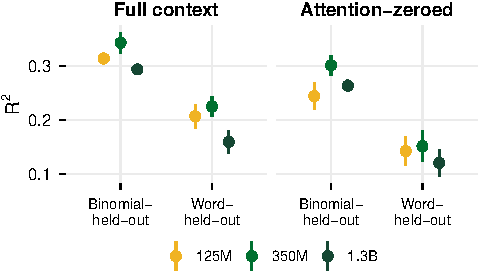
\includegraphics[keepaspectratio]{writeup_files/figure-pdf/fig-r2-babylm-1.pdf}}

}

\caption{\label{fig-r2-babylm}Cross-validated probe R² at the final
hidden layer for the BabyLM models, binomial level, by attention
condition. Bars = ±1 SD across 10 folds (minimum width enforced for
visibility). The drop from the left to the right of each panel is the
lexical generalization cost.}

\end{figure}%

For the binomial-level conditions, binomial-held-out R² ranges from 0.24
to 0.34; word-held-out R² is consistently lower, ranging from 0.12 to
0.23. The drop reflects a lexical generalization cost: the probe is more
accurate when a test binomial's words appeared in other training
binomials than when both are novel, so some preference signal is tied to
word identity rather than being fully abstract. Probe accuracy is
non-monotonic with model size, and the full-context condition yields
higher binomial-held-out R² than attention-zeroed, a difference we
report but do not build on.

\subsubsection{Abstract and Stored
Contributions}\label{abstract-and-stored-contributions}

Both sources predict the model's ordering preference, and both do so
credibly in all three models. Under full context, \(\hat{y}\) carries a
coefficient between +0.332 and +0.434, and \(r\) one between +0.221 and
+0.341, with 95\% credible intervals excluding zero throughout
(Appendix~\ref{sec-appendix-relfreq}). A BabyLM's preference for an
attested binomial is thus governed partly by what generalizes from
binomials it never saw, and partly by the order its own corpus happens
to attest for that specific pair. Neither alone accounts for the
ordering.

Attention-zeroing separates the two. Blocking cross-word attention
reduces the contribution of the corpus's attested order by 9--26\%,
against 7--17\% for the abstract component. The two ranges overlap, but
the asymmetry holds within each model taken separately: the attested
order loses more than the abstract component does in all three. Since
the zeroed representation is additive in the two words and can carry no
information about them jointly, the component that gives way is the one
that required them to interact.

The frequency moderation is present here too. The attested order gains
ground with exposure in all three models (+0.115 {[}+0.107, +0.124{]},
+0.104 {[}+0.095, +0.113{]} and +0.103 {[}+0.094, +0.111{]}), and in
each case that gain is roughly halved under attention-zeroing (+0.055,
+0.060 and +0.034). These are the same magnitudes the large-scale models
show in Experiment 2, so the models trained on a human-scale corpus need
no separate account: the frequency-dependent trade-off appears at 100M
tokens and does not require web-scale exposure to emerge. The caveat is
on precision rather than direction. 70\% of BabyLM's binomials occur
exactly once, so \(r\) sits at a boundary value for most of the set and
its lowest frequency deciles consist entirely of singletons, leaving the
measure coarse at the low-frequency end
(Appendix~\ref{sec-appendix-relfreq}). Experiment 2 supplies the
frequency range these models lack.

\begin{figure}

\centering{

\pandocbounded{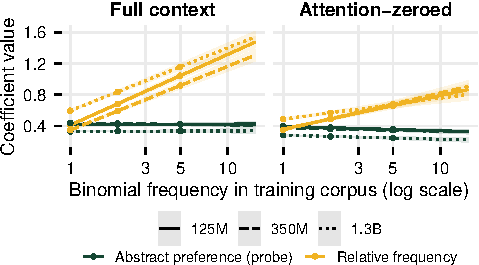
\includegraphics[keepaspectratio]{writeup_files/figure-pdf/fig-relfreq-babylm-1.pdf}}

}

\caption{\label{fig-relfreq-babylm}How strongly each source contributes
to the BabyLM models' ordering preference, by binomial frequency. Values
are simple slopes from the fitted posteriors of
Equation~\ref{eq-relfreq}, evaluated at each decile's median frequency
and plotted against that frequency. The lines are straight because
Equation~\ref{eq-relfreq} is linear in \texttt{log\_freq}, so a simple
slope is exactly linear in it; points mark the decile medians, and their
spacing shows where the binomials actually are. Bands are 95\% credible
intervals, widest at the extremes because a simple slope is least
precisely estimated far from the mean. Under full context relative
frequency gains ground as frequency rises while the abstract component
loses it; under attention-zeroing relative frequency sits lower
throughout.}

\end{figure}%

\section{Experiment 2: Cross-Family Final-Layer
Representations}\label{sec-exp2}

Experiment 1 demonstrates that BabyLMs rely on both abstract preferences
and holistic storage for binomial ordering. Those models are small in
both parameters and training data, so Experiment 2 applies the same
probe to 13 further models across four large-scale families: Pythia,
GPT-2, OLMo, and Llama, with the BabyLM results carried over for
comparison (Appendix~\ref{sec-appendix-models}).

\subsection{Results}\label{results-1}

\subsubsection{Probe Performance}\label{probe-performance-1}

Figure~\ref{fig-r2} shows both cross-validation splits for all 16
models; full numbers, control probes, and the word-level replication are
in Appendix~\ref{sec-appendix-exp2}. Control R² was near zero throughout
(mean ± SD = 0.0002 ± 0.0002). All large-scale models substantially
outperform BabyLM: full-context binomial-held-out R² spans 0.43 to 0.65
against 0.29--0.34, and word-held-out R² is lower than binomial-held-out
for every model and condition. Attention-zeroing raises
binomial-held-out R² in every large-scale family, most sharply in GPT-2,
where it reaches 0.79 at 117M against 0.65 under full context;
Llama-3-8B is the sole exception. Scale effects within families are
non-monotonic, with GPT-2 R² \emph{decreasing} with size, from 0.65 at
117M to 0.49 at XL.

\begin{figure*}

\centering{

\pandocbounded{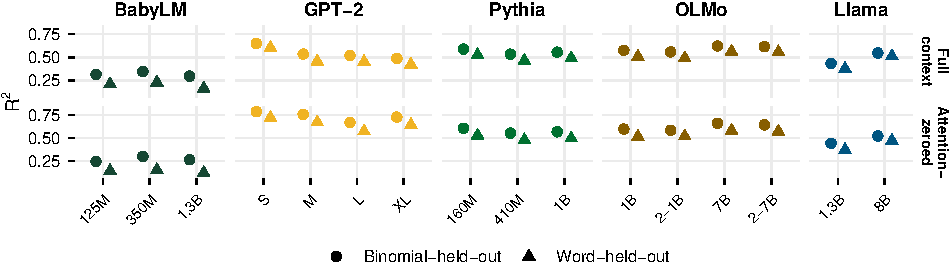
\includegraphics[keepaspectratio]{writeup_files/figure-pdf/fig-r2-1.pdf}}

}

\caption{\label{fig-r2}Cross-validated R² for all 16 models, by
attention condition and cross-validation split. Circles =
binomial-held-out; triangles = word-held-out. Bars = 95\% CI across 10
folds. Models ordered by parameter count within each family and colored
by family. Control R² \(\approx\) 0 (Appendix~\ref{sec-appendix-exp2}).}

\end{figure*}%

\subsubsection{Abstract and Stored
Contributions}\label{abstract-and-stored-contributions-1}

The frequency range BabyLM lacks sharpens the moderation and separates
the two moderators. Under full context, the contribution of the corpus's
attested order grows with exposure in all 13 large-scale models, and the
abstract component's shrinks in all 13, with 95\% credible intervals
excluding zero in every case (Table~\ref{tbl-relfreq};
Figure~\ref{fig-relfreq-coefs}). The two moderators run in opposite
directions on the same items: the more often a model saw a binomial, the
more its ordering is governed by that binomial's own attested order and
the less by what generalizes from binomials it never saw.

The effect is substantial rather than marginal. In GPT-2 the two sources
cross over: the attested order's standardized slope climbs from 0.05 in
the rarest frequency decile to 0.51 in the most frequent, while the
abstract component's falls from 0.51 to 0.47, so that for the most
frequent binomials the corpus's own attested order is the better
predictor of the two (Figure~\ref{fig-relfreq-pile}). The crossing is
not universal: in Llama-3-8B the attested order climbs from 0.11 to 0.40
while the abstract component falls from 0.67 to 0.55, converging without
meeting. The direction is the same in every model; whether the two
actually cross depends on where each starts.

Attention-zeroing removes this selectively, which is what identifies
where the stored component lives. The attested order's contribution
falls by 40--70\% across the large-scale models, and its moderation by
frequency falls by roughly 72\% alongside it, though it remains credible
in 13 of 13 models rather than vanishing outright. The abstract
component moves the other way: it is \emph{larger} under
attention-zeroing in every one of the 13, by 5--43\%. Since the zeroed
representation is additive in the two words, no information about them
jointly can reach the probe, so what the intervention strips is the
component that required the two words to be encoded together. A blunt
degradation of the representation would have reduced both terms; this
reduces one and raises the other. It is worth being clear about what
remains: roughly half of the attested order's contribution survives an
additive representation, so the item-specific knowledge is not carried
by a pair representation alone. Experiment 3 shows this surviving
portion is the part that appears first, and Section~\ref{sec-discussion}
takes up what it is likely to be.

One term does not behave as the storage account predicts. The abstract
component's moderation stays negative under attention-zeroing in all 13
large-scale models rather than flattening, so its decline with frequency
is not caused by stored orderings displacing it. The probe is trained on
novel binomials, which by construction have no corpus frequency; the
words of frequent attested binomials have had their representations
shaped by those binomial contexts, and a mapping learned from nonce
items transfers less well to them. That is a claim about lexical
representations rather than phrasal storage, and the intervention leaves
it intact because word-additive representations survive the mask.

\begin{figure}[t]

\centering{

\pandocbounded{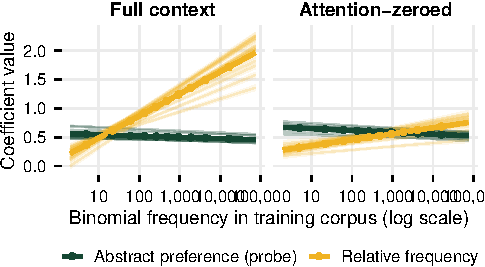
\includegraphics[keepaspectratio]{writeup_files/figure-pdf/fig-relfreq-pile-1.pdf}}

}

\caption{\label{fig-relfreq-pile}How strongly each source contributes to
the ordering preference, by binomial frequency, for the 13 large-scale
models. Values are simple slopes from the fitted posteriors of
Equation~\ref{eq-relfreq}, evaluated at each decile's median frequency
and plotted against that frequency; faint lines are individual models
with their 95\% credible intervals, bold lines their mean. The lines are
straight because Equation~\ref{eq-relfreq} is linear in
\texttt{log\_freq}. Under full context the abstract component weakens
and relative frequency strengthens in all 13; the two cross in Pythia,
GPT-2 and Llama-1.3B but not in OLMo or Llama-3-8B. Under
attention-zeroing relative frequency sits far lower throughout.}

\end{figure}%

\section{Experiment 3: Developmental Trajectories}\label{sec-exp3}

Experiments 1 and 2 establish that language models encode binomial
preferences at the end of training, but leave open when those
representations emerge, and whether the trade-off between abstract
preferences and holistic storage is present early or accumulates with
exposure. Experiment 3 examines the same probe at multiple training
checkpoints.

The probe, input modes, attention conditions, and cross-validation
splits are as described in Section~\ref{sec-methods}. We refit
Equation~\ref{eq-relfreq} at each saved checkpoint of the three BabyLM
models and the three Pythia models for which checkpoints were available,
in both attention conditions: 72 fits in all. Because every variable is
standardized within each fit, coefficients are comparable across
checkpoints as well as across models.

The two sets of checkpoints cover very different portions of training
and should not be read as a common axis. BabyLM's six steps span roughly
the first two-thirds of its run, whereas Pythia's stop at step 1000 of
about 143,000, or the first 0.7\%. Pythia therefore shows what happens
very early, and its final-checkpoint models from Experiment 2 show where
that leads, with nothing in between.

\subsection{Results}\label{results-2}

Probe trajectories are shown in Figure~\ref{fig-checkpoints} and the two
sources' contributions in Figure~\ref{fig-ckpt-sources}. BabyLM
binomial-held-out R² is already high at the earliest checkpoint
(\textasciitilde20M tokens: 0.67--0.72) and broadly declines to
0.32--0.38 by the end of training. At the earliest checkpoint, the
attention-zeroed condition outperforms full context (0.78--0.80
vs.~0.67--0.72); this ordering reverses between \textasciitilde120M and
\textasciitilde750M tokens, so that full context exceeds
attention-zeroed at the final checkpoint for all three model sizes.
Pythia shows an inverted-U trajectory instead: R² rises from 0.68--0.74
at 33.6M tokens to a peak of 0.80--0.86 at 537M tokens, then declines to
0.71--0.76 at 1074M--2097M tokens, consistent with large-scale models
still consolidating preference representations during this early window
(the first 0.7\% of 300B tokens). The attention condition flip for
Pythia follows the same qualitative pattern as BabyLM. Full numerical
and word-level results are in Appendix~\ref{sec-appendix-exp3}.

The stored contribution accumulates. Across the first three checkpoints
\texttt{rel\_freq} is negligible in every model, never exceeding 0.034
in absolute value and credibly different from zero in only 19 of 36
cells, in both directions. From the fourth checkpoint it is credibly
positive in 36 of 36 model-by-condition cells and climbs thereafter: to
0.224, 0.200 and 0.387 in the three BabyLM models and to 0.140, 0.140
and 0.152 in the three Pythia models. This holds in both attention
conditions, so what grows is not solely the part that requires the two
words to interact. Item-specific ordering information is not present
from the outset; it is acquired, and it keeps accruing for as long as we
can observe.

What the intervention removes appears later than the contribution
itself, and the lag is informative. At the fourth checkpoint, the first
at which \texttt{rel\_freq} is credibly positive in every model,
attention-zeroing removes none of it: the gap between conditions is
0.025 at most and as often slightly negative as positive, in both
corpora and on both terms. Item-specific ordering information is
therefore already measurable at a point where it survives a strictly
additive representation intact. Whatever carries it at this stage is not
holistic storage, which by definition requires the pair: it is the
individual lexical representations.

Holistic storage then accumulates on top of it. The share of
\texttt{rel\_freq} that attention-zeroing removes rises from nothing at
the fourth checkpoint to 20--23\% by the last in the three Pythia models
and 8--24\% in the three BabyLM models, and reaches 40--70\% in the
fully trained large-scale models. The frequency moderation follows the
same course, its condition gap reaching 0.041, 0.030 and 0.085 in BabyLM
and 0.037, 0.029 and 0.038 in Pythia. Repeated exposure to a binomial
thus leaves item-specific knowledge in two forms, and they arrive in
order: first in the lexical representations, and only later as holistic
storage. The abstract component moves independently of all this.
\texttt{y\_pred} declines steadily across BabyLM training in both
conditions (0.625 to 0.428 in BabyLM-125M under full context) while
rising over Pythia's early window and then falling below its starting
value by the final model (0.528 at step 16, 0.686 at step 256, 0.462
fully trained). Its moderation,
\texttt{y\_pred}\(\times\)\texttt{log\_freq}, is credibly negative under
attention-zeroing in 26 of the 36 checkpoint cells, but with no trend
common to the two corpora: it drifts further from zero across BabyLM
training and back toward zero across Pythia's. Full numerical results
are in Appendix~\ref{sec-appendix-exp3}.

\begin{figure}

\centering{

\pandocbounded{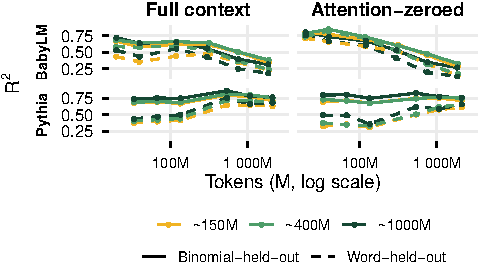
\includegraphics[keepaspectratio]{writeup_files/figure-pdf/fig-checkpoints-1.pdf}}

}

\caption{\label{fig-checkpoints}Cross-validated probe R² across BabyLM
and Pythia training checkpoints, by attention condition and
cross-validation split. BabyLM's checkpoints span most of its training
run, Pythia's only the first 0.7\% of its own, so the two x-axes are not
on a common footing. Control R² \(\approx\) 0.}

\end{figure}%

\begin{figure}

\centering{

\pandocbounded{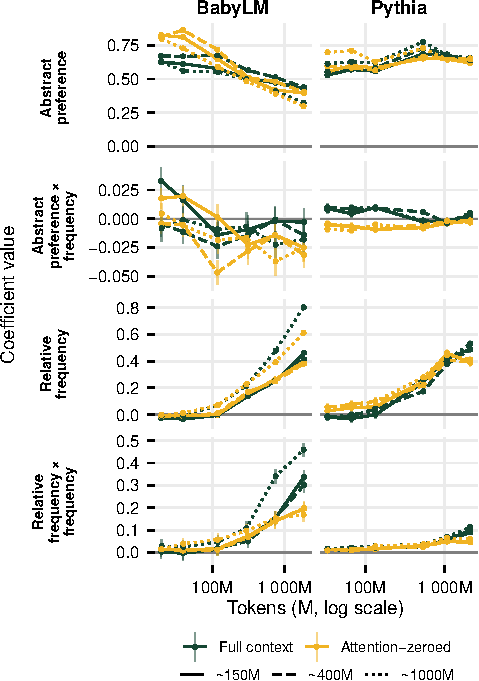
\includegraphics[keepaspectratio]{writeup_files/figure-pdf/fig-ckpt-sources-1.pdf}}

}

\caption{\label{fig-ckpt-sources}All four terms of
Equation~\ref{eq-relfreq} across training, with 95\% credible intervals.
Rows are the two sources and their moderations by frequency, on separate
y-scales because they occupy very different ranges; color marks the
attention condition and linetype the model size. All variables are
standardized within each fit, so values are comparable across
checkpoints and models. The abstract component is substantial from the
earliest checkpoint while the attested order starts near zero and
accumulates. The two conditions track each other on the main effects
until the final checkpoints; they separate most clearly on the attested
order's moderation (bottom row), where attention-zeroing roughly halves
the coefficient by the end of training in every model. The abstract
component's moderation stays near zero throughout and shows no trend
common to the two corpora. Neither the y-axes nor the x-axes are on a
common footing across panels: BabyLM's checkpoints span most of its
training run, Pythia's only the first 0.7\% of its own.}

\end{figure}%

\section{Discussion and Conclusion}\label{sec-discussion}

The present study examined whether language models' binomial ordering
preferences are driven by abstract structure, and if so, how that
structure emerges throughout training. Across 16 models from five
families, we found that ordering preferences are recoverable and
generalize to unseen words, that a model's preference for an attested
binomial is governed jointly by what generalizes from binomials it never
saw and by the order its own corpus attests for that particular pair,
that the balance between the two shifts toward the attested order as a
binomial becomes more frequent, and that zeroing out cross-word
attention removes roughly half of the attested-order contribution in the
large-scale models while the abstract one survives, growing rather than
shrinking in every one of them.

Ordering preferences are therefore clearly driven by abstract
preferences. The probe recovers a model's preference for binomials built
entirely from words it was never trained on, which is not something a
lookup of stored items can do, and a ridge probe with a single tuned
hyperparameter recovers the same pattern, so the result does not depend
on the MLP's capacity (Appendix~\ref{sec-appendix-linear}), and the
answer to the question left open by \citet{houghton2025role} is that
models do have abstract preferences, but ones a test for human
constraints failed to detect. Further evidence that these preferences
are systematic rather than an arbitrary consequence of the weights is
established without the probe at all: independently trained models
converge on the same preferences for the same novel binomials
(\(r = 0.45\), against a shuffled baseline of \(r \approx 0.00\)),
including the three BabyLM models, which share a training corpus but
differ in capacity. Agreement is also higher within a family than
between families, which rules out the shared sentence frame as its
source: the frame is identical for all sixteen models, so it could not
produce such a gap. At the same time, a binomial's own attested order
contributes over and above anything the abstract mapping supplies, and
contributes more the more often the model saw it. That contribution is
item-specific by construction: it is a fact about one pair of words, not
a constraint that generalizes. This is the same trade-off between
abstract preferences and holistic storage that \citet{morgan2016} found
in humans, emerging in a system that does not have them innately encoded
in them.

The developmental trajectory separates the two components in time.
Abstract preferences are present very early: probe R² is already high at
the earliest BabyLM checkpoint, at roughly 20M tokens, and the abstract
component of Equation~\ref{eq-relfreq} is large from the first
checkpoint in every model. The stored contribution is not. It is
negligible through the first three checkpoints of every model, becomes
credibly positive everywhere from the fourth, and climbs monotonically
thereafter under full context, without levelling off. Item-specific
ordering information is therefore acquired rather than present from the
outset, and it is still accumulating at the last point we can observe.
What the intervention removes grows too, and it lags the contribution
itself. At the first checkpoint where a binomial's attested order
predicts the model's preference at all, attention-zeroing removes none
of that prediction; the share it removes then climbs to roughly half by
the end of training. Item-specific ordering knowledge therefore arrives
in the lexical representations before it arrives as holistic storage.

Usage-based accounts have long held that frequently encountered
expressions become stored and retrieved as units rather than assembled
from their parts, and behavioral work on binomials has shown that human
ordering preferences reflect both abstract constraints and direct
experience with particular items. The present study corroborates these
accounts in a system with no innate linguistic preferences at all: the
same frequency-dependent trade-off emerges in a distributed network
trained only to predict text, suggesting that it need not be built in,
and can emerge from exposure alone. Zeroing out cross-word attention
then shows where the stored component lives. Because the intervention
makes the representation additive in the two words, it can carry nothing
about them jointly, and what it removes is drawn specifically from the
contribution of the binomial's own attested order. What it does
\emph{not} remove is equally informative. Roughly half of that
contribution survives an additive representation, and it is not, at
least, the part the probe's abstract prediction already explains, since
that prediction is a covariate in the same fit and is computed from the
same additive representation. The probe is not a complete account of
abstract structure, so some of what survives may be generalizable
knowledge it failed to recover. The more interesting possibility is that
repeated exposure to a binomial in its own frame shifts the
representations of its individual words, so that a word encountered
overwhelmingly in first position comes to encode something of that
tendency on its own. That is still item-specific knowledge, a fact about
particular words rather than a constraint that generalizes, but it is
not holistic storage: it has been distilled into the lexical
representations and no longer needs the pair. On this reading,
entrenchment yields item-specific knowledge in two forms rather than
one, and the developmental data orders them: the lexical form is present
as soon as the attested order predicts anything at all, and holistic
storage accumulates afterwards. The trade-off \citet{morgan2016}
describe in humans is then not a single dial between abstract
preferences and holistic storage, but a sequence, with the lexicon
carrying the earliest item-specific knowledge and the pair
representation taking over later. The abstract component survives the
same intervention: it is \emph{larger} under attention-zeroing in all 13
large-scale models, by 5--43\%, and smaller by only 7--17\% in the three
BabyLM models. A representation that had merely been degraded would have
lost both. Repeated exposure does not simply add a stored preference
alongside an abstract one: it builds something that requires the two
words to be encoded together, and that can be switched off without
disturbing what generalizes.

\section*{Limitations}\label{limitations}
\addcontentsline{toc}{section}{Limitations}

The novel binomials were selected to be absent from BabyLM's training
corpus, so they are genuinely novel only for the three BabyLM models;
indexed against Dolma \citep{dolma}, a trillion-token corpus, roughly
98.4\% occur at non-zero frequency. For the thirteen large-scale models
the probe is therefore trained on infrequent attested binomials rather
than unseen ones. This is why Experiment 1 anchors the interpretation:
the inference that a recovered preference must have been generalized
rather than retrieved rests on BabyLM, and the larger models extend that
pattern rather than establish it. Corpus frequency is likewise an exact
measure of what the model saw only for BabyLM and Pythia; for GPT-2,
OLMo, and Llama, Pile counts stand in as a proxy for web-scale exposure.

The stored-ordering measure is estimated from counts, so it is least
reliable exactly where exposure is lowest. A binomial seen once takes
the same boundary value as one seen a thousand times in a single order,
which makes the predictor coarse for rare items and attenuates its
coefficient there. The effect is strongest for BabyLM, where most items
sit at a boundary and the measure is close to binary, and mild for the
large-scale models, where it varies continuously through its range. That
the two return moderation estimates of similar size argues against the
coefficient being mostly an artifact of saturation, but attenuation and
growing storage do push it in the same direction, so part of any
positive estimate reflects improving measurement. This is why we read
the comparison between attention conditions rather than the moderation
on its own, since the counts, and therefore the attenuation, are
identical in both conditions and cancel from the difference.

Separately, BabyLM and Pythia deliver cumulative exposure to individual
binomials at nearly the same rate per training token, so total text read
and per-binomial exposure cannot be told apart here; distinguishing them
would require matched models trained on repeated versus varied text.

Probe performance establishes that ordering information is present in a
model's representations and recoverable by a mapping that generalizes to
unseen words, but not that the model uses that information in the way
the probe reads it. Our central claims are accordingly framed as
differences between attention conditions and across frequency strata
rather than as inferences from absolute decodability, and the
attention-zeroed quantity is guaranteed by the architecture rather than
estimated by the probe. This distinction does real work: a
representation that merely carried the outcome of the computation would
be read equally well at every frequency, predicting neither a shift in
which source governs the ordering nor any change in that shift when
cross-word attention is blocked, and both are observed in every
large-scale model. Overall R² does also differ between the two attention
conditions in a direction that is not stable across families or across
training, and we draw no conclusions from it.

Finally, the results are limited to English and to a single
construction, and checkpoints were available for two of the five
families, so the developmental claims rest on BabyLM and Pythia. Whether
attention-zeroing separates per-word from relational information as
cleanly in constructions with a different structure is untested, though
the argument that it should is architectural rather than empirical and
does not depend on properties peculiar to binomials.

\bibliography{references}
\clearpage

\onecolumn

\appendix

% Appendix layout. Two separate things are going on here.
%
% \raggedbottom is the important one. acl.sty sets \flushbottom, which forces
% every page to exact height by stretching the flexible glue between paragraphs
% and around headings. On an appendix page that cannot fill naturally, that
% stretch becomes a gap in the middle of the page with text stranded above and
% below it. \raggedbottom instead lets the slack collect at the foot of the
% page, which is the conventional choice for appendix matter. Main-text pages
% keep \flushbottom and the two-column look.
%
% Tables are not floats here at all: every appendix table is emitted as a
% longtable, which typesets inline and breaks across pages. That is what keeps
% them exactly where they are declared. A float cannot do this: Table 9 alone
% is about 640pt against a 706pt text block, so as a float it could never share
% a page with the heading and prose that introduce it, and [H] simply pushed it
% to the next page and left the previous one blank.
%
% Figures are still floats and are pinned with [H], which is fine because none
% of them needs to break across a page.
\raggedbottom
\floatplacement{figure}{H}

\section{Model Details}\label{sec-appendix-models}

Table \ref{tbl-models} lists all 16 models used across experiments,
organized by family, with approximate parameter counts and training
token counts.

\begingroup\fontsize{9}{11}\selectfont

\begin{longtable}[t]{llll}

\toprule
Family & Model & Parameters & Tokens\\
\midrule
\endfirsthead
\multicolumn{4}{@{}l}{\textit{(continued)}}\\
\toprule
Family & Model & Parameters & Tokens\\
\midrule
\endhead

\endfoot
\bottomrule
\endlastfoot
 & BabyLM-125M & 125M & 150M\\
\nopagebreak
 & BabyLM-350M & 350M & 150M\\
\nopagebreak
\multirow{-3}{*}{\raggedright\arraybackslash BabyLM} & BabyLM-1.3B & 1.3B & 150M\\
\cmidrule{1-4}\pagebreak[0]
 & GPT-2 & 117M & \textasciitilde{}8B\\
\nopagebreak
 & GPT-2-medium & 345M & \textasciitilde{}8B\\
\nopagebreak
 & GPT-2-large & 762M & \textasciitilde{}8B\\
\nopagebreak
\multirow{-4}{*}{\raggedright\arraybackslash GPT-2} & GPT-2-XL & 1.5B & \textasciitilde{}8B\\
\cmidrule{1-4}\pagebreak[0]
 & Pythia-160M & 160M & \textasciitilde{}300B\\
\nopagebreak
 & Pythia-410M & 410M & \textasciitilde{}300B\\
\nopagebreak
\multirow{-3}{*}{\raggedright\arraybackslash Pythia} & Pythia-1B & 1B & \textasciitilde{}300B\\
\cmidrule{1-4}\pagebreak[0]
 & OLMo-1B & 1B & 3T\\
\nopagebreak
 & OLMo-7B & 7B & 2.5T\\
\nopagebreak
 & OLMo-2-1B & 1B & \textasciitilde{}4T\\
\nopagebreak
\multirow{-4}{*}{\raggedright\arraybackslash OLMo} & OLMo-2-7B & 7B & \textasciitilde{}4T\\
\cmidrule{1-4}\pagebreak[0]
 & Llama-1.3B & 1.2B & \textasciitilde{}9T\\
\nopagebreak
\multirow{-2}{*}{\raggedright\arraybackslash Llama} & Llama-3-8B & 8B & \textasciitilde{}15T\\*


\caption{\label{tbl-models}Models used across experiments. Training
token counts for full-scale models are approximate; GPT-2 counts are
estimated from the reported 40GB WebText corpus. BabyLM models train for
20 epochs over 150M tokens (3B effective token exposures).}

\tabularnewline
\end{longtable}

\endgroup{}

\clearpage

\section{Binomial Extraction Criteria}\label{sec-appendix-extraction}

Candidate ``\(W_1\) and \(W_2\)'' sequences were first selected using
spaCy \citep{spacy2} part-of-speech tags, retaining only cases where
both \(W_1\) and \(W_2\) are open-class words (nouns, verbs, adjectives,
or adverbs). Each candidate was then parsed with the Berkeley Neural
Parser
\citep{kitaev-klein-2018-constituency, kitaev-etal-2019-multilingual} to
confirm that the two words form a minimal coordinate phrase. The
inclusion criterion was that the two words be co-constituents under the
same phrasal node (NP, VP, ADJP, ADVP, PP, or equivalent), with that
node spanning exactly the three tokens {[}\(W_1\), and, \(W_2\){]} and
nothing else. This ensures the extracted items are genuine coordinate
binomials rather than incidental sequences where ``and'' links clauses
or longer phrases. Novel binomials were extracted from Wikitext by the
identical procedure, with the added requirements that both words appear
in BabyLM's vocabulary and that the binomial is absent from the attested
set.

Because cross-category coordination is syntactically unacceptable,
violating the Coordination of Likes constraint that benepar enforces
through its Penn Treebank training, genuine mixed-category binomials are
excluded by the constituency criterion rather than by any explicit POS
filter. We deliberately avoid filtering by spaCy POS tag agreement
because spaCy frequently misclassifies participial forms in coordinate
contexts, for example tagging ``mortified'' as VERB rather than ADJ in
``disgusted and mortified.'' Explicit POS filtering would therefore
discard many valid same-category binomials without catching any genuine
cross-category ones.

\clearpage

\section{Implementation Details}\label{sec-appendix-implementation}

\textbf{Probe training.} The probe is optimized with Adam (learning rate
\(10^{-3}\), weight decay \(10^{-4}\)) under mean-squared-error loss,
with early stopping (patience 20) against a 10\% held-out validation
split. Antisymmetric augmentation is applied with probability 0.5: for
each binomial the flipped version, with swapped ordering and negated
label, is added to the training batch. The input dimensionality follows
from the representation type as defined in Section~\ref{sec-methods}.

\textbf{Attention-zeroing.} The mask is supplied to the model as a 4D
attention mask rather than a 2D padding mask, so it applies at every
transformer layer rather than only the first. This matters because a
mask applied at the first layer alone would leave \(W_2\) able to
recover information about \(W_1\) indirectly at greater depth, through
positions that did attend to it.

\textbf{Recomputing the target.} Because \(y_{true}\) is the model's own
log-probability ratio, it is recomputed from whichever forward pass
produced the representations being probed. The two full-context
representation types therefore share a target, while the
attention-zeroed condition has its own: blocking cross-word attention
changes the model's output probabilities as well as its hidden states.
Each attention condition is thus a self-consistent probe problem rather
than two input encodings evaluated against a fixed target.

\clearpage

\section{Linear Probe Replication}\label{sec-appendix-linear}

The MLP probe has many free choices: hidden dimension, depth,
activation, learning rate, weight decay, patience, validation fraction,
augmentation probability, batch size, and initialization. A skeptical
reading is that some of them were tuned toward the reported result. We
therefore repeat the analysis with a probe that has one.

The linear probe is a ridge regression on the same antisymmetric
features, fit on the same cross-validation folds. It has no intercept,
since the antisymmetric feature is odd by construction and the target
has zero mean at the origin, and no optimization schedule, since the
solution is closed-form. Its only free quantity is the ridge penalty,
selected per fold from \(\{10^0, \ldots, 10^5\}\) on an inner split of
that fold's training data. That inner split is the same size as the
MLP's early-stopping split, so both probes receive an identical budget
of held-out data for hyperparameter selection.

Across 52 model-checkpoint cells and 207 comparisons, the two probes
agree closely (\emph{r} = 0.928 between their R² values). On the
word-held-out split the linear probe recovers 86\% of the MLP's R² on
average (0.410 vs.~0.476).

\begingroup\fontsize{8}{10}\selectfont

\begin{longtable}[t]{llllll}

\toprule
Model & Condition & Split & Linear & MLP & Gap\\
\midrule
\endfirsthead
\multicolumn{6}{@{}l}{\textit{(continued)}}\\
\toprule
Model & Condition & Split & Linear & MLP & Gap\\
\midrule
\endhead

\endfoot
\bottomrule
\endlastfoot
 &  & B & 0.169 & 0.244 & +0.075\\
\nopagebreak
 & \multirow{-2}{*}{\raggedright\arraybackslash Attention-zeroed} & W & 0.103 & 0.143 & +0.040\\
\nopagebreak
 &  & B & 0.197 & 0.314 & +0.116\\
\nopagebreak
\multirow{-4}{*}[0.5\dimexpr\aboverulesep+\belowrulesep+\cmidrulewidth]{\raggedright\arraybackslash BabyLM-125m} & \multirow{-2}{*}{\raggedright\arraybackslash Full context} & W & 0.147 & 0.207 & +0.060\\
\cmidrule{1-6}\pagebreak[0]
 &  & B & 0.185 & 0.263 & +0.078\\
\nopagebreak
 & \multirow{-2}{*}{\raggedright\arraybackslash Attention-zeroed} & W & 0.094 & 0.121 & +0.027\\
\nopagebreak
 &  & B & 0.188 & 0.294 & +0.105\\
\nopagebreak
\multirow{-4}{*}[0.5\dimexpr\aboverulesep+\belowrulesep+\cmidrulewidth]{\raggedright\arraybackslash BabyLM-1\_3b} & \multirow{-2}{*}{\raggedright\arraybackslash Full context} & W & 0.127 & 0.160 & +0.032\\
\cmidrule{1-6}\pagebreak[0]
 &  & B & 0.211 & 0.301 & +0.090\\
\nopagebreak
 & \multirow{-2}{*}{\raggedright\arraybackslash Attention-zeroed} & W & 0.121 & 0.152 & +0.031\\
\nopagebreak
 &  & B & 0.223 & 0.343 & +0.120\\
\nopagebreak
\multirow{-4}{*}[0.5\dimexpr\aboverulesep+\belowrulesep+\cmidrulewidth]{\raggedright\arraybackslash BabyLM-350m} & \multirow{-2}{*}{\raggedright\arraybackslash Full context} & W & 0.170 & 0.225 & +0.055\\
\cmidrule{1-6}\pagebreak[0]
 &  & B & 0.336 & 0.443 & +0.107\\
\nopagebreak
 & \multirow{-2}{*}{\raggedright\arraybackslash Attention-zeroed} & W & 0.288 & 0.370 & +0.082\\
\nopagebreak
 &  & B & 0.357 & 0.433 & +0.076\\
\nopagebreak
\multirow{-4}{*}[0.5\dimexpr\aboverulesep+\belowrulesep+\cmidrulewidth]{\raggedright\arraybackslash Llama-3.2-1B} & \multirow{-2}{*}{\raggedright\arraybackslash Full context} & W & 0.332 & 0.373 & +0.041\\
\cmidrule{1-6}\pagebreak[0]
 &  & B & 0.465 & 0.521 & +0.057\\
\nopagebreak
 & \multirow{-2}{*}{\raggedright\arraybackslash Attention-zeroed} & W & 0.420 & 0.470 & +0.050\\
\nopagebreak
 &  & B & 0.507 & 0.545 & +0.038\\
\nopagebreak
\multirow{-4}{*}[0.5\dimexpr\aboverulesep+\belowrulesep+\cmidrulewidth]{\raggedright\arraybackslash Meta-Llama-3-8B} & \multirow{-2}{*}{\raggedright\arraybackslash Full context} & W & 0.485 & 0.510 & +0.026\\
\cmidrule{1-6}\pagebreak[0]
 &  & B & 0.482 & 0.597 & +0.114\\
\nopagebreak
 & \multirow{-2}{*}{\raggedright\arraybackslash Attention-zeroed} & W & 0.438 & 0.514 & +0.076\\
\nopagebreak
 &  & B & 0.466 & 0.575 & +0.108\\
\nopagebreak
\multirow{-4}{*}[0.5\dimexpr\aboverulesep+\belowrulesep+\cmidrulewidth]{\raggedright\arraybackslash OLMo-1B-hf} & \multirow{-2}{*}{\raggedright\arraybackslash Full context} & W & 0.439 & 0.505 & +0.066\\
\cmidrule{1-6}\pagebreak[0]
 &  & B & 0.477 & 0.583 & +0.105\\
\nopagebreak
 & \multirow{-2}{*}{\raggedright\arraybackslash Attention-zeroed} & W & 0.448 & 0.518 & +0.070\\
\nopagebreak
 &  & B & 0.460 & 0.557 & +0.096\\
\nopagebreak
\multirow{-4}{*}[0.5\dimexpr\aboverulesep+\belowrulesep+\cmidrulewidth]{\raggedright\arraybackslash OLMo-2-0425-1B} & \multirow{-2}{*}{\raggedright\arraybackslash Full context} & W & 0.438 & 0.488 & +0.051\\
\cmidrule{1-6}\pagebreak[0]
 &  & B & 0.566 & 0.642 & +0.076\\
\nopagebreak
 & \multirow{-2}{*}{\raggedright\arraybackslash Attention-zeroed} & W & 0.525 & 0.570 & +0.044\\
\nopagebreak
 &  & B & 0.559 & 0.614 & +0.055\\
\nopagebreak
\multirow{-4}{*}[0.5\dimexpr\aboverulesep+\belowrulesep+\cmidrulewidth]{\raggedright\arraybackslash OLMo-2-1124-7B} & \multirow{-2}{*}{\raggedright\arraybackslash Full context} & W & 0.531 & 0.554 & +0.023\\
\cmidrule{1-6}\pagebreak[0]
 &  & B & 0.575 & 0.658 & +0.083\\
\nopagebreak
 & \multirow{-2}{*}{\raggedright\arraybackslash Attention-zeroed} & W & 0.518 & 0.580 & +0.062\\
\nopagebreak
 &  & B & 0.553 & 0.621 & +0.067\\
\nopagebreak
\multirow{-4}{*}[0.5\dimexpr\aboverulesep+\belowrulesep+\cmidrulewidth]{\raggedright\arraybackslash OLMo-7B-hf} & \multirow{-2}{*}{\raggedright\arraybackslash Full context} & W & 0.518 & 0.561 & +0.043\\
\cmidrule{1-6}\pagebreak[0]
 &  & B & 0.647 & 0.786 & +0.139\\
\nopagebreak
 & \multirow{-2}{*}{\raggedright\arraybackslash Attention-zeroed} & W & 0.606 & 0.718 & +0.111\\
\nopagebreak
 &  & B & 0.569 & 0.648 & +0.079\\
\nopagebreak
\multirow{-4}{*}[0.5\dimexpr\aboverulesep+\belowrulesep+\cmidrulewidth]{\raggedright\arraybackslash gpt2} & \multirow{-2}{*}{\raggedright\arraybackslash Full context} & W & 0.556 & 0.601 & +0.045\\
\cmidrule{1-6}\pagebreak[0]
 &  & B & 0.523 & 0.668 & +0.145\\
\nopagebreak
 & \multirow{-2}{*}{\raggedright\arraybackslash Attention-zeroed} & W & 0.468 & 0.571 & +0.103\\
\nopagebreak
 &  & B & 0.414 & 0.519 & +0.105\\
\nopagebreak
\multirow{-4}{*}[0.5\dimexpr\aboverulesep+\belowrulesep+\cmidrulewidth]{\raggedright\arraybackslash gpt2-large} & \multirow{-2}{*}{\raggedright\arraybackslash Full context} & W & 0.392 & 0.449 & +0.057\\
\cmidrule{1-6}\pagebreak[0]
 &  & B & 0.621 & 0.756 & +0.136\\
\nopagebreak
 & \multirow{-2}{*}{\raggedright\arraybackslash Attention-zeroed} & W & 0.567 & 0.670 & +0.103\\
\nopagebreak
 &  & B & 0.396 & 0.533 & +0.138\\
\nopagebreak
\multirow{-4}{*}[0.5\dimexpr\aboverulesep+\belowrulesep+\cmidrulewidth]{\raggedright\arraybackslash gpt2-medium} & \multirow{-2}{*}{\raggedright\arraybackslash Full context} & W & 0.373 & 0.453 & +0.081\\
\cmidrule{1-6}\pagebreak[0]
 &  & B & 0.609 & 0.726 & +0.117\\
\nopagebreak
 & \multirow{-2}{*}{\raggedright\arraybackslash Attention-zeroed} & W & 0.560 & 0.641 & +0.081\\
\nopagebreak
 &  & B & 0.394 & 0.487 & +0.092\\
\nopagebreak
\multirow{-4}{*}[0.5\dimexpr\aboverulesep+\belowrulesep+\cmidrulewidth]{\raggedright\arraybackslash gpt2-xl} & \multirow{-2}{*}{\raggedright\arraybackslash Full context} & W & 0.369 & 0.420 & +0.051\\
\cmidrule{1-6}\pagebreak[0]
 &  & B & 0.481 & 0.604 & +0.122\\
\nopagebreak
 & \multirow{-2}{*}{\raggedright\arraybackslash Attention-zeroed} & W & 0.456 & 0.527 & +0.071\\
\nopagebreak
 &  & B & 0.459 & 0.587 & +0.128\\
\nopagebreak
\multirow{-4}{*}[0.5\dimexpr\aboverulesep+\belowrulesep+\cmidrulewidth]{\raggedright\arraybackslash pythia-160m} & \multirow{-2}{*}{\raggedright\arraybackslash Full context} & W & 0.445 & 0.522 & +0.077\\
\cmidrule{1-6}\pagebreak[0]
 &  & B & 0.479 & 0.567 & +0.088\\
\nopagebreak
 & \multirow{-2}{*}{\raggedright\arraybackslash Attention-zeroed} & W & 0.437 & 0.496 & +0.058\\
\nopagebreak
 &  & B & 0.471 & 0.554 & +0.083\\
\nopagebreak
\multirow{-4}{*}[0.5\dimexpr\aboverulesep+\belowrulesep+\cmidrulewidth]{\raggedright\arraybackslash pythia-1b} & \multirow{-2}{*}{\raggedright\arraybackslash Full context} & W & 0.440 & 0.488 & +0.048\\
\cmidrule{1-6}\pagebreak[0]
 &  & B & 0.434 & 0.552 & +0.118\\
\nopagebreak
 & \multirow{-2}{*}{\raggedright\arraybackslash Attention-zeroed} & W & 0.407 & 0.477 & +0.070\\
\nopagebreak
 &  & B & 0.413 & 0.532 & +0.118\\
\nopagebreak
\multirow{-4}{*}[0.5\dimexpr\aboverulesep+\belowrulesep+\cmidrulewidth]{\raggedright\arraybackslash pythia-410m} & \multirow{-2}{*}{\raggedright\arraybackslash Full context} & W & 0.392 & 0.461 & +0.069\\*


\caption{\label{tbl-linear}Linear (ridge) versus MLP probe R² at the
final hidden layer, binomial-level input mode. Both probes use identical
cross-validation folds. B = binomial-held-out; W = word-held-out. Gap =
MLP minus linear.}

\tabularnewline
\end{longtable}

\endgroup{}

The gap between the probes is consistently larger on the
binomial-held-out split than on the word-held-out split. This is
expected: binomial-held-out performance is partly recoverable from word
identity alone, which a flexible model can exploit and a linear map on
the same features cannot. Word-held-out performance, on which the
paper's claims rest, is where the two agree most closely.

\clearpage

\section{Cross-Validation Split Sizes}\label{sec-appendix-cv}

Cross-validation is carried out on the novel set only. The attested set
is never cross-validated: it is used solely as the transfer target
described in Section~\ref{sec-methods-analyses}, where a probe trained
on the full novel set predicts every attested binomial and those
predictions enter the ordering-source regression as \(\hat{y}\). Both
splits use ten folds with seed 964, and the same folds are reused across
models, attention conditions, and probe architectures so that all
reported R² values are directly comparable.

Under the binomial-held-out split, binomials are assigned to folds
directly, so each fold trains on nine tenths of the set and tests on the
remaining tenth. Under the word-held-out split it is the
\emph{vocabulary} that is partitioned into ten folds. A binomial enters
the test set for fold \(k\) only if both of its words are in fold \(k\),
and enters the training set only if neither word is. Binomials with one
word in fold \(k\) and one word outside it are used in neither, and are
discarded for that fold. Since a binomial needs both words drawn from
the same tenth of the vocabulary to be testable, the word-held-out test
set is roughly a hundredth of the set rather than a tenth.
Table~\ref{tbl-cv-sizes} gives the resulting sizes.

\begingroup\fontsize{9}{11}\selectfont

\begin{longtable}[t]{llll}

\toprule
Split & Train / fold & Test / fold & Discarded / fold\\
\midrule
\endfirsthead
\multicolumn{4}{@{}l}{\textit{(continued)}}\\
\toprule
Split & Train / fold & Test / fold & Discarded / fold\\
\midrule
\endhead

\endfoot
\bottomrule
\endlastfoot
Binomial-held-out & 306,038 & 34,004 & 0\\
Word-held-out & 271,560--279,306 & 3,086--3,839 & 61,101 (18.0\%)\\*


\caption{\label{tbl-cv-sizes}Cross-validation fold sizes for the novel
set (340,042 binomials over 50,137 unique words). Ranges are across the
10 folds. Discarded items under word-held-out are binomials with exactly
one word in the held-out vocabulary fold.}

\tabularnewline
\end{longtable}

\endgroup{}

No fold under either split fell below the minimum test-set size of 10
binomials required for a fold to be scored, so all ten folds contribute
to every reported mean. For reference, the attested set to which the
trained probe is transferred contains 48,965 binomials over 21,721
unique words, all of which receive a prediction.

\clearpage

\section{Experiment 1: Supplementary Results}\label{sec-appendix-exp1}

This appendix provides supplementary materials for Experiment 1
(§\ref{sec-exp1}), which examined final-layer probe performance for the
three BabyLM models. Subsections report full R² tables, control probe
results, and a word-level replication. Coefficients for the
ordering-source regression are reported together for all models in
Appendix~\ref{sec-appendix-relfreq}.

\subsection{Full Probe R²}\label{sec-appendix-full-r2-babylm}

Probe R² at the final hidden layer for BabyLM models, at the binomial
level by attention condition. B = binomial-held-out; W = word-held-out.
SD across 10 folds in parentheses.

\begingroup\fontsize{8}{10}\selectfont

\begin{longtable}[t]{lllll}

\toprule
Model & Condition & Split & R² & Ctrl\\
\midrule
\endfirsthead
\multicolumn{5}{@{}l}{\textit{(continued)}}\\
\toprule
Model & Condition & Split & R² & Ctrl\\
\midrule
\endhead

\endfoot
\bottomrule
\endlastfoot
 &  & B & 0.314 (0.010) & 0.000 (0.000)\\
\nopagebreak
 & \multirow{-2}{*}{\raggedright\arraybackslash Full context} & W & 0.207 (0.023) & 0.000 (0.000)\\
\nopagebreak
 &  & B & 0.244 (0.025) & 0.000 (0.000)\\
\nopagebreak
\multirow{-4}{*}[0.5\dimexpr\aboverulesep+\belowrulesep+\cmidrulewidth]{\raggedright\arraybackslash BabyLM-125M} & \multirow{-2}{*}{\raggedright\arraybackslash Attention-zeroed} & W & 0.143 (0.027) & 0.000 (0.000)\\
\cmidrule{1-5}\pagebreak[0]
 &  & B & 0.343 (0.019) & 0.000 (0.000)\\
\nopagebreak
 & \multirow{-2}{*}{\raggedright\arraybackslash Full context} & W & 0.225 (0.018) & 0.000 (0.000)\\
\nopagebreak
 &  & B & 0.301 (0.019) & 0.000 (0.000)\\
\nopagebreak
\multirow{-4}{*}[0.5\dimexpr\aboverulesep+\belowrulesep+\cmidrulewidth]{\raggedright\arraybackslash BabyLM-350M} & \multirow{-2}{*}{\raggedright\arraybackslash Attention-zeroed} & W & 0.152 (0.028) & 0.000 (0.000)\\
\cmidrule{1-5}\pagebreak[0]
 &  & B & 0.294 (0.004) & 0.000 (0.000)\\
\nopagebreak
 & \multirow{-2}{*}{\raggedright\arraybackslash Full context} & W & 0.160 (0.022) & 0.000 (0.000)\\
\nopagebreak
 &  & B & 0.263 (0.012) & 0.000 (0.000)\\
\nopagebreak
\multirow{-4}{*}[0.5\dimexpr\aboverulesep+\belowrulesep+\cmidrulewidth]{\raggedright\arraybackslash BabyLM-1.3B} & \multirow{-2}{*}{\raggedright\arraybackslash Attention-zeroed} & W & 0.121 (0.025) & 0.000 (0.000)\\*


\caption{\label{tbl-r2-babylm}Probe R² at the final hidden layer for
BabyLM models, at the binomial level by attention condition. B =
binomial-held-out split; W = word-held-out split. SD across 10 folds in
parentheses.}

\tabularnewline
\end{longtable}

\endgroup{}

\subsection{Control Probe R²}\label{sec-appendix-ctrl-exp1}

Control probe R² for BabyLM models at the final hidden layer, at the
binomial level by attention condition. Labels are randomly permuted;
values near zero confirm the main probe recovers genuine linguistic
structure rather than label artifacts or probe capacity.

\begingroup\fontsize{8}{10}\selectfont

\begin{longtable}[t]{llll}

\toprule
Model & Condition & Split & Control R²\\
\midrule
\endfirsthead
\multicolumn{4}{@{}l}{\textit{(continued)}}\\
\toprule
Model & Condition & Split & Control R²\\
\midrule
\endhead

\endfoot
\bottomrule
\endlastfoot
 &  & B & 0.0000 (0.0000)\\
\nopagebreak
 & \multirow{-2}{*}{\raggedright\arraybackslash Attention-zeroed} & W & 0.0005 (0.0005)\\
\nopagebreak
 &  & B & 0.0001 (0.0001)\\
\nopagebreak
\multirow{-4}{*}[0.5\dimexpr\aboverulesep+\belowrulesep+\cmidrulewidth]{\raggedright\arraybackslash BabyLM-125M} & \multirow{-2}{*}{\raggedright\arraybackslash Full context} & W & 0.0002 (0.0002)\\
\cmidrule{1-4}\pagebreak[0]
 &  & B & 0.0000 (0.0000)\\
\nopagebreak
 & \multirow{-2}{*}{\raggedright\arraybackslash Attention-zeroed} & W & 0.0001 (0.0001)\\
\nopagebreak
 &  & B & 0.0000 (0.0000)\\
\nopagebreak
\multirow{-4}{*}[0.5\dimexpr\aboverulesep+\belowrulesep+\cmidrulewidth]{\raggedright\arraybackslash BabyLM-350M} & \multirow{-2}{*}{\raggedright\arraybackslash Full context} & W & 0.0002 (0.0002)\\
\cmidrule{1-4}\pagebreak[0]
 &  & B & 0.0000 (0.0000)\\
\nopagebreak
 & \multirow{-2}{*}{\raggedright\arraybackslash Attention-zeroed} & W & 0.0001 (0.0001)\\
\nopagebreak
 &  & B & 0.0000 (0.0001)\\
\nopagebreak
\multirow{-4}{*}[0.5\dimexpr\aboverulesep+\belowrulesep+\cmidrulewidth]{\raggedright\arraybackslash BabyLM-1.3B} & \multirow{-2}{*}{\raggedright\arraybackslash Full context} & W & 0.0002 (0.0002)\\*


\caption{\label{tbl-ctrl-r2-babylm}Control probe R² for BabyLM models
(final layer), at the binomial level by attention condition. SD across
10 folds in parentheses. B = binomial-held-out; W = word-held-out.}

\tabularnewline
\end{longtable}

\endgroup{}

\subsection{Cross-Model Agreement on Novel
Binomials}\label{sec-appendix-agreement}

A binomial absent from the training corpus cannot have a retrieved
preference, but the model still assigns one, and that value is some
deterministic function of the two words' representations. Such a
function could reflect systematic knowledge, or it could be an arbitrary
consequence of a particular set of weights. Probe generalization cannot
distinguish these, because both are systematic functions of the input
and both transfer to held-out words. Agreement between independently
trained models can: an arbitrary function of one model's weights has no
reason to match another's.

We therefore correlate \(y_{true}\) across models on identical
binomials, separately for the attested and novel sets and for both
attention conditions. As a baseline we shuffle one model's values, which
removes any pairing between models while preserving both distributions.

The three BabyLM models are the decisive comparison. They share a
training corpus and its ordering but differ in capacity, and they are
the only models for which the novel binomials are genuinely absent from
training (Section~\ref{sec-exp2}, Methods). On novel binomials they
agree at \(r = 0.45\) under full context and \(r = 0.41\) under
attention-zeroing, against a shuffled baseline of \(r \approx 0.00\).
Preferences for binomials the models never encountered are therefore
reproducible across models of different sizes trained on the same data,
which rules out their being arbitrary.

Because a Pearson correlation can in principle be carried by a minority
of high-magnitude items, we checked whether the agreement is
concentrated in strong preferences while the bulk of binomials agree at
chance. It is not. Preferences on novel binomials are not weak to begin
with: median \(|y_{true}|\) ranges from 1.79 to 3.21 across the three
models, so the preferred ordering is between roughly six and twenty-five
times more likely, and only 9\% to 17\% of binomials fall below 0.5.
Rank correlations track the Pearson values closely (0.371--0.406 for
BabyLM on novel binomials), and the models order the same binomial the
same way on 60\% to 70\% of items against a chance rate of 50\%, a
statistic that ignores magnitude and weights every binomial equally.
Stratifying by preference strength, using the third model's
\(|y_{true}|\) so that the bins are independent of the two series being
correlated, agreement is graded but present throughout: in the weakest
quintile \(r = 0.30\) under full context and \(0.28\) under
attention-zeroing, with directional agreement near 59\% in both, rising
to \(r = 0.61\) and 73\% in the strongest. That gradient is itself
informative, since agreement increasing with preference strength is the
signature of a signal measured with noise rather than of an arbitrary
function of a particular set of weights.

Two further patterns appear in Table~\ref{tbl-agreement}. Agreement
within a family is roughly constant across all four cells, near
\(r = 0.68\), whereas agreement between families falls from 0.56 on
attested binomials under full context to 0.28 on novel binomials under
attention-zeroing. What the models share thus survives novelty when the
training corpus is shared and degrades when it is not, as expected if
the preference is driven by distributional structure in the training
data. This also rules out the shared sentence frame as the source of the
agreement: the frame is identical for all sixteen models, so it cannot
produce a gap between within-family and between-family agreement.

\begingroup\fontsize{8}{10}\selectfont

\begin{longtable}[t]{lllll}

\toprule
Set & Condition & Scope & $r$ & Shuffled\\
\midrule
\endfirsthead
\multicolumn{5}{@{}l}{\textit{(continued)}}\\
\toprule
Set & Condition & Scope & $r$ & Shuffled\\
\midrule
\endhead

\endfoot
\bottomrule
\endlastfoot
 &  & All & 0.470 & -0.003\\
\nopagebreak
 &  & Within family & 0.680 & -0.003\\
\nopagebreak
 &  & Between family & 0.431 & -0.003\\
\nopagebreak
 & \multirow{-4}{*}{\raggedright\arraybackslash Attention-zeroed} & Within BabyLM & 0.508 & -0.003\\
\nopagebreak
 &  & All & 0.583 & -0.003\\
\nopagebreak
 &  & Within family & 0.721 & -0.003\\
\nopagebreak
 &  & Between family & 0.557 & -0.003\\
\nopagebreak
\multirow{-8}{*}[0.5\dimexpr\aboverulesep+\belowrulesep+\cmidrulewidth]{\raggedright\arraybackslash Attested} & \multirow{-4}{*}{\raggedright\arraybackslash Full context} & Within BabyLM & 0.553 & -0.003\\
\cmidrule{1-5}\pagebreak[0]
 &  & All & 0.346 & 0.000\\
\nopagebreak
 &  & Within family & 0.683 & 0.000\\
\nopagebreak
 &  & Between family & 0.283 & 0.000\\
\nopagebreak
 & \multirow{-4}{*}{\raggedright\arraybackslash Attention-zeroed} & Within BabyLM & 0.408 & 0.000\\
\nopagebreak
 &  & All & 0.447 & -0.002\\
\nopagebreak
 &  & Within family & 0.679 & -0.002\\
\nopagebreak
 &  & Between family & 0.403 & -0.002\\
\nopagebreak
\multirow{-8}{*}[0.5\dimexpr\aboverulesep+\belowrulesep+\cmidrulewidth]{\raggedright\arraybackslash Novel} & \multirow{-4}{*}{\raggedright\arraybackslash Full context} & Within BabyLM & 0.452 & -0.002\\*


\caption{\label{tbl-agreement}Cross-model agreement (Pearson \(r\) on
\(y_{true}\)) for identical binomials, by item set and attention
condition. Shuffled = one model's values permuted. Within-family
averages over model pairs from the same family; BabyLM is broken out
because its novel binomials are genuinely unseen.}

\tabularnewline
\end{longtable}

\endgroup{}

\subsection{Word-Level Replication}\label{sec-appendix-words-only-exp1}

We trained the MLP probe using word-level representations for the three
BabyLM models to verify that the preference signal is not an artifact of
mean pooling across the full binomial phrase. Under this condition the
probe receives a concatenation of two word vectors extracted from
isolated sentence contexts (``\emph{the bread}'', ``\emph{the
butter}''), so it cannot rely on any co-occurrence signal from the two
words' shared sentence context.

Binomial-held-out R² ranges from 0.31 to 0.33, within a few percentage
points of the corresponding binomial-level values (0.29--0.34). The
generalization pattern is preserved: word-held-out R² is consistently
lower than binomial-held-out R² for all three models (word-held-out
0.18--0.20; binomial-minus-word gap 0.127--0.129), confirming that the
lexical generalization cost seen at the binomial level is a property of
the preference encoding itself rather than an artifact of the
mean-pooled representation. The ordering-source regression was fit at
the binomial level only, so it has no word-level counterpart. Full
results are in Table~\ref{tbl-r2-babylm-words-only}.

\begingroup\fontsize{8}{10}\selectfont

\begin{longtable}[t]{llllll}

\toprule
Model & Mode & Split & R² & Ctrl & Sel.\\
\midrule
\endfirsthead
\multicolumn{6}{@{}l}{\textit{(continued)}}\\
\toprule
Model & Mode & Split & R² & Ctrl & Sel.\\
\midrule
\endhead

\endfoot
\bottomrule
\endlastfoot
 &  & B & 0.312 (0.012) & 0.000 (0.000) & 0.312\\
\nopagebreak
\multirow{-2}{*}{\raggedright\arraybackslash BabyLM-125M} &  & W & 0.185 (0.015) & 0.000 (0.000) & 0.184\\
 &  & B & 0.326 (0.010) & 0.000 (0.000) & 0.326\\
\nopagebreak
\multirow{-2}{*}{\raggedright\arraybackslash BabyLM-350M} &  & W & 0.199 (0.016) & 0.000 (0.000) & 0.198\\
 &  & B & 0.306 (0.003) & 0.000 (0.000) & 0.306\\
\nopagebreak
\multirow{-2}{*}{\raggedright\arraybackslash BabyLM-1.3B} & \multirow{-6}{*}{\raggedright\arraybackslash Word-level} & W & 0.177 (0.023) & 0.000 (0.000) & 0.177\\*


\caption{\label{tbl-r2-babylm-words-only}Word-level probe R² and
selectivity (main \(-\) control R²) for BabyLM models (final layer). B =
binomial-held-out split; W = word-held-out split. SD across 10 folds in
parentheses.}

\tabularnewline
\end{longtable}

\endgroup{}

\section{Experiment 2: Supplementary Results}\label{sec-appendix-exp2}

This appendix provides supplementary materials for Experiment 2
(§\ref{sec-exp2}), which examined final-layer representations across all
16 models from five families. Subsections report full R² tables, control
probe results, and a word-level replication. Coefficients for the
ordering-source regression are in Appendix~\ref{sec-appendix-relfreq}.

\subsection{Full Probe R²}\label{sec-appendix-full-r2}

Probe R² for all 16 models at the final hidden layer, binomial-level
input mode, by attention condition and cross-validation split. B =
binomial-held-out; W = word-held-out. SD across 10 folds in parentheses.

\begingroup\fontsize{7}{9}\selectfont

\begin{longtable}[t]{lllll}

\toprule
Model & Condition & Split & R² & Ctrl\\
\midrule
\endfirsthead
\multicolumn{5}{@{}l}{\textit{(continued)}}\\
\toprule
Model & Condition & Split & R² & Ctrl\\
\midrule
\endhead

\endfoot
\bottomrule
\endlastfoot
 &  & B & 0.314 (0.010) & 0.000 (0.000)\\
\nopagebreak
 & \multirow{-2}{*}{\raggedright\arraybackslash Full context} & W & 0.207 (0.023) & 0.000 (0.000)\\
\nopagebreak
 &  & B & 0.244 (0.025) & 0.000 (0.000)\\
\nopagebreak
\multirow{-4}{*}[0.5\dimexpr\aboverulesep+\belowrulesep+\cmidrulewidth]{\raggedright\arraybackslash BabyLM-125M} & \multirow{-2}{*}{\raggedright\arraybackslash Attention-zeroed} & W & 0.143 (0.027) & 0.000 (0.000)\\
\cmidrule{1-5}\pagebreak[0]
 &  & B & 0.343 (0.019) & 0.000 (0.000)\\
\nopagebreak
 & \multirow{-2}{*}{\raggedright\arraybackslash Full context} & W & 0.225 (0.018) & 0.000 (0.000)\\
\nopagebreak
 &  & B & 0.301 (0.019) & 0.000 (0.000)\\
\nopagebreak
\multirow{-4}{*}[0.5\dimexpr\aboverulesep+\belowrulesep+\cmidrulewidth]{\raggedright\arraybackslash BabyLM-350M} & \multirow{-2}{*}{\raggedright\arraybackslash Attention-zeroed} & W & 0.152 (0.028) & 0.000 (0.000)\\
\cmidrule{1-5}\pagebreak[0]
 &  & B & 0.294 (0.004) & 0.000 (0.000)\\
\nopagebreak
 & \multirow{-2}{*}{\raggedright\arraybackslash Full context} & W & 0.160 (0.022) & 0.000 (0.000)\\
\nopagebreak
 &  & B & 0.263 (0.012) & 0.000 (0.000)\\
\nopagebreak
\multirow{-4}{*}[0.5\dimexpr\aboverulesep+\belowrulesep+\cmidrulewidth]{\raggedright\arraybackslash BabyLM-1.3B} & \multirow{-2}{*}{\raggedright\arraybackslash Attention-zeroed} & W & 0.121 (0.025) & 0.000 (0.000)\\
\cmidrule{1-5}\pagebreak[0]
 &  & B & 0.648 (0.004) & 0.000 (0.000)\\
\nopagebreak
 & \multirow{-2}{*}{\raggedright\arraybackslash Full context} & W & 0.601 (0.033) & 0.001 (0.001)\\
\nopagebreak
 &  & B & 0.786 (0.006) & 0.000 (0.000)\\
\nopagebreak
\multirow{-4}{*}[0.5\dimexpr\aboverulesep+\belowrulesep+\cmidrulewidth]{\raggedright\arraybackslash GPT-2} & \multirow{-2}{*}{\raggedright\arraybackslash Attention-zeroed} & W & 0.718 (0.024) & 0.000 (0.000)\\
\cmidrule{1-5}\pagebreak[0]
 &  & B & 0.533 (0.005) & 0.000 (0.000)\\
\nopagebreak
 & \multirow{-2}{*}{\raggedright\arraybackslash Full context} & W & 0.453 (0.028) & 0.000 (0.000)\\
\nopagebreak
 &  & B & 0.756 (0.016) & 0.000 (0.000)\\
\nopagebreak
\multirow{-4}{*}[0.5\dimexpr\aboverulesep+\belowrulesep+\cmidrulewidth]{\raggedright\arraybackslash GPT-2-M} & \multirow{-2}{*}{\raggedright\arraybackslash Attention-zeroed} & W & 0.670 (0.036) & 0.000 (0.000)\\
\cmidrule{1-5}\pagebreak[0]
 &  & B & 0.519 (0.006) & 0.000 (0.000)\\
\nopagebreak
 & \multirow{-2}{*}{\raggedright\arraybackslash Full context} & W & 0.449 (0.036) & 0.000 (0.000)\\
\nopagebreak
 &  & B & 0.668 (0.006) & 0.000 (0.000)\\
\nopagebreak
\multirow{-4}{*}[0.5\dimexpr\aboverulesep+\belowrulesep+\cmidrulewidth]{\raggedright\arraybackslash GPT-2-L} & \multirow{-2}{*}{\raggedright\arraybackslash Attention-zeroed} & W & 0.571 (0.020) & 0.000 (0.000)\\
\cmidrule{1-5}\pagebreak[0]
 &  & B & 0.487 (0.007) & 0.000 (0.000)\\
\nopagebreak
 & \multirow{-2}{*}{\raggedright\arraybackslash Full context} & W & 0.420 (0.033) & 0.000 (0.000)\\
\nopagebreak
 &  & B & 0.726 (0.008) & 0.000 (0.000)\\
\nopagebreak
\multirow{-4}{*}[0.5\dimexpr\aboverulesep+\belowrulesep+\cmidrulewidth]{\raggedright\arraybackslash GPT-2-XL} & \multirow{-2}{*}{\raggedright\arraybackslash Attention-zeroed} & W & 0.641 (0.034) & 0.000 (0.000)\\
\cmidrule{1-5}\pagebreak[0]
 &  & B & 0.587 (0.005) & 0.000 (0.000)\\
\nopagebreak
 & \multirow{-2}{*}{\raggedright\arraybackslash Full context} & W & 0.522 (0.021) & 0.000 (0.000)\\
\nopagebreak
 &  & B & 0.604 (0.005) & 0.000 (0.000)\\
\nopagebreak
\multirow{-4}{*}[0.5\dimexpr\aboverulesep+\belowrulesep+\cmidrulewidth]{\raggedright\arraybackslash Pythia-160M} & \multirow{-2}{*}{\raggedright\arraybackslash Attention-zeroed} & W & 0.527 (0.022) & 0.001 (0.001)\\
\cmidrule{1-5}\pagebreak[0]
 &  & B & 0.532 (0.004) & 0.000 (0.000)\\
\nopagebreak
 & \multirow{-2}{*}{\raggedright\arraybackslash Full context} & W & 0.461 (0.035) & 0.000 (0.000)\\
\nopagebreak
 &  & B & 0.552 (0.006) & 0.000 (0.000)\\
\nopagebreak
\multirow{-4}{*}[0.5\dimexpr\aboverulesep+\belowrulesep+\cmidrulewidth]{\raggedright\arraybackslash Pythia-410M} & \multirow{-2}{*}{\raggedright\arraybackslash Attention-zeroed} & W & 0.477 (0.019) & 0.000 (0.000)\\
\cmidrule{1-5}\pagebreak[0]
 &  & B & 0.554 (0.007) & 0.000 (0.000)\\
\nopagebreak
 & \multirow{-2}{*}{\raggedright\arraybackslash Full context} & W & 0.488 (0.029) & 0.000 (0.000)\\
\nopagebreak
 &  & B & 0.567 (0.005) & 0.000 (0.000)\\
\nopagebreak
\multirow{-4}{*}[0.5\dimexpr\aboverulesep+\belowrulesep+\cmidrulewidth]{\raggedright\arraybackslash Pythia-1B} & \multirow{-2}{*}{\raggedright\arraybackslash Attention-zeroed} & W & 0.496 (0.027) & 0.000 (0.000)\\
\cmidrule{1-5}\pagebreak[0]
 &  & B & 0.575 (0.005) & 0.000 (0.000)\\
\nopagebreak
 & \multirow{-2}{*}{\raggedright\arraybackslash Full context} & W & 0.505 (0.021) & 0.000 (0.000)\\
\nopagebreak
 &  & B & 0.597 (0.008) & 0.000 (0.000)\\
\nopagebreak
\multirow{-4}{*}[0.5\dimexpr\aboverulesep+\belowrulesep+\cmidrulewidth]{\raggedright\arraybackslash OLMo-1B} & \multirow{-2}{*}{\raggedright\arraybackslash Attention-zeroed} & W & 0.514 (0.021) & 0.000 (0.000)\\
\cmidrule{1-5}\pagebreak[0]
 &  & B & 0.621 (0.008) & 0.000 (0.000)\\
\nopagebreak
 & \multirow{-2}{*}{\raggedright\arraybackslash Full context} & W & 0.561 (0.023) & 0.000 (0.000)\\
\nopagebreak
 &  & B & 0.658 (0.008) & 0.000 (0.000)\\
\nopagebreak
\multirow{-4}{*}[0.5\dimexpr\aboverulesep+\belowrulesep+\cmidrulewidth]{\raggedright\arraybackslash OLMo-7B} & \multirow{-2}{*}{\raggedright\arraybackslash Attention-zeroed} & W & 0.580 (0.027) & 0.000 (0.000)\\
\cmidrule{1-5}\pagebreak[0]
 &  & B & 0.557 (0.007) & 0.000 (0.000)\\
\nopagebreak
 & \multirow{-2}{*}{\raggedright\arraybackslash Full context} & W & 0.488 (0.017) & 0.000 (0.000)\\
\nopagebreak
 &  & B & 0.583 (0.005) & 0.000 (0.000)\\
\nopagebreak
\multirow{-4}{*}[0.5\dimexpr\aboverulesep+\belowrulesep+\cmidrulewidth]{\raggedright\arraybackslash OLMo-2-1B} & \multirow{-2}{*}{\raggedright\arraybackslash Attention-zeroed} & W & 0.518 (0.021) & 0.000 (0.000)\\
\cmidrule{1-5}\pagebreak[0]
 &  & B & 0.614 (0.005) & 0.000 (0.000)\\
\nopagebreak
 & \multirow{-2}{*}{\raggedright\arraybackslash Full context} & W & 0.554 (0.022) & 0.000 (0.000)\\
\nopagebreak
 &  & B & 0.642 (0.006) & 0.000 (0.000)\\
\nopagebreak
\multirow{-4}{*}[0.5\dimexpr\aboverulesep+\belowrulesep+\cmidrulewidth]{\raggedright\arraybackslash OLMo-2-7B} & \multirow{-2}{*}{\raggedright\arraybackslash Attention-zeroed} & W & 0.570 (0.012) & 0.000 (0.000)\\
\cmidrule{1-5}\pagebreak[0]
 &  & B & 0.433 (0.008) & 0.000 (0.000)\\
\nopagebreak
 & \multirow{-2}{*}{\raggedright\arraybackslash Full context} & W & 0.373 (0.035) & 0.000 (0.000)\\
\nopagebreak
 &  & B & 0.443 (0.011) & 0.000 (0.000)\\
\nopagebreak
\multirow{-4}{*}[0.5\dimexpr\aboverulesep+\belowrulesep+\cmidrulewidth]{\raggedright\arraybackslash Llama-1.3B} & \multirow{-2}{*}{\raggedright\arraybackslash Attention-zeroed} & W & 0.370 (0.040) & 0.000 (0.000)\\
\cmidrule{1-5}\pagebreak[0]
 &  & B & 0.545 (0.008) & 0.000 (0.000)\\
\nopagebreak
 & \multirow{-2}{*}{\raggedright\arraybackslash Full context} & W & 0.510 (0.035) & 0.001 (0.001)\\
\nopagebreak
 &  & B & 0.521 (0.016) & 0.000 (0.000)\\
\nopagebreak
\multirow{-4}{*}[0.5\dimexpr\aboverulesep+\belowrulesep+\cmidrulewidth]{\raggedright\arraybackslash Llama-3-8B} & \multirow{-2}{*}{\raggedright\arraybackslash Attention-zeroed} & W & 0.470 (0.024) & 0.000 (0.000)\\*


\caption{\label{tbl-r2}Probe R² at the final hidden layer for all 16
models, at the binomial level by attention condition. B =
binomial-held-out split; W = word-held-out split. SD across 10 folds in
parentheses.}

\tabularnewline
\end{longtable}

\endgroup{}

\subsection{Control Probe R²}\label{sec-appendix-ctrl-exp2}

Control probe R² for all 16 models at the final hidden layer, at the
binomial level by attention condition.

\begingroup\fontsize{8}{10}\selectfont

\begin{longtable}[t]{lllll}

\toprule
Family & Model & Condition & Split & Control R²\\
\midrule
\endfirsthead
\multicolumn{5}{@{}l}{\textit{(continued)}}\\
\toprule
Family & Model & Condition & Split & Control R²\\
\midrule
\endhead

\endfoot
\bottomrule
\endlastfoot
 &  &  & B & 0.0000 (0.0000)\\
\nopagebreak
 &  & \multirow{-2}{*}{\raggedright\arraybackslash Attention-zeroed} & W & 0.0005 (0.0005)\\
\nopagebreak
 &  &  & B & 0.0001 (0.0001)\\
\nopagebreak
 & \multirow{-4}{*}[0.5\dimexpr\aboverulesep+\belowrulesep+\cmidrulewidth]{\raggedright\arraybackslash BabyLM-125M} & \multirow{-2}{*}{\raggedright\arraybackslash Full context} & W & 0.0002 (0.0002)\\
\nopagebreak
 &  &  & B & 0.0000 (0.0000)\\
\nopagebreak
 &  & \multirow{-2}{*}{\raggedright\arraybackslash Attention-zeroed} & W & 0.0001 (0.0001)\\
\nopagebreak
 &  &  & B & 0.0000 (0.0000)\\
\nopagebreak
 & \multirow{-4}{*}[0.5\dimexpr\aboverulesep+\belowrulesep+\cmidrulewidth]{\raggedright\arraybackslash BabyLM-350M} & \multirow{-2}{*}{\raggedright\arraybackslash Full context} & W & 0.0002 (0.0002)\\
\nopagebreak
 &  &  & B & 0.0000 (0.0000)\\
\nopagebreak
 &  & \multirow{-2}{*}{\raggedright\arraybackslash Attention-zeroed} & W & 0.0001 (0.0001)\\
\nopagebreak
 &  &  & B & 0.0000 (0.0001)\\
\nopagebreak
\multirow{-12}{*}[2.5\dimexpr\aboverulesep+\belowrulesep+\cmidrulewidth]{\raggedright\arraybackslash BabyLM} & \multirow{-4}{*}[0.5\dimexpr\aboverulesep+\belowrulesep+\cmidrulewidth]{\raggedright\arraybackslash BabyLM-1.3B} & \multirow{-2}{*}{\raggedright\arraybackslash Full context} & W & 0.0002 (0.0002)\\
\cmidrule{1-5}\pagebreak[0]
 &  &  & B & 0.0000 (0.0000)\\
\nopagebreak
 &  & \multirow{-2}{*}{\raggedright\arraybackslash Attention-zeroed} & W & 0.0001 (0.0001)\\
\nopagebreak
 &  &  & B & 0.0000 (0.0000)\\
\nopagebreak
 & \multirow{-4}{*}[0.5\dimexpr\aboverulesep+\belowrulesep+\cmidrulewidth]{\raggedright\arraybackslash GPT-2} & \multirow{-2}{*}{\raggedright\arraybackslash Full context} & W & 0.0005 (0.0006)\\
\nopagebreak
 &  &  & B & 0.0000 (0.0000)\\
\nopagebreak
 &  & \multirow{-2}{*}{\raggedright\arraybackslash Attention-zeroed} & W & 0.0002 (0.0003)\\
\nopagebreak
 &  &  & B & 0.0000 (0.0000)\\
\nopagebreak
 & \multirow{-4}{*}[0.5\dimexpr\aboverulesep+\belowrulesep+\cmidrulewidth]{\raggedright\arraybackslash GPT-2-M} & \multirow{-2}{*}{\raggedright\arraybackslash Full context} & W & 0.0002 (0.0002)\\
\nopagebreak
 &  &  & B & 0.0000 (0.0000)\\
\nopagebreak
 &  & \multirow{-2}{*}{\raggedright\arraybackslash Attention-zeroed} & W & 0.0004 (0.0005)\\
\nopagebreak
 &  &  & B & 0.0000 (0.0000)\\
\nopagebreak
 & \multirow{-4}{*}[0.5\dimexpr\aboverulesep+\belowrulesep+\cmidrulewidth]{\raggedright\arraybackslash GPT-2-L} & \multirow{-2}{*}{\raggedright\arraybackslash Full context} & W & 0.0003 (0.0004)\\
\nopagebreak
 &  &  & B & 0.0000 (0.0000)\\
\nopagebreak
 &  & \multirow{-2}{*}{\raggedright\arraybackslash Attention-zeroed} & W & 0.0003 (0.0004)\\
\nopagebreak
 &  &  & B & 0.0000 (0.0000)\\
\nopagebreak
\multirow{-16}{*}[3.5\dimexpr\aboverulesep+\belowrulesep+\cmidrulewidth]{\raggedright\arraybackslash GPT-2} & \multirow{-4}{*}[0.5\dimexpr\aboverulesep+\belowrulesep+\cmidrulewidth]{\raggedright\arraybackslash GPT-2-XL} & \multirow{-2}{*}{\raggedright\arraybackslash Full context} & W & 0.0002 (0.0003)\\
\cmidrule{1-5}\pagebreak[0]
 &  &  & B & 0.0000 (0.0000)\\
\nopagebreak
 &  & \multirow{-2}{*}{\raggedright\arraybackslash Attention-zeroed} & W & 0.0002 (0.0003)\\
\nopagebreak
 &  &  & B & 0.0000 (0.0000)\\
\nopagebreak
 & \multirow{-4}{*}[0.5\dimexpr\aboverulesep+\belowrulesep+\cmidrulewidth]{\raggedright\arraybackslash Llama-1.3B} & \multirow{-2}{*}{\raggedright\arraybackslash Full context} & W & 0.0003 (0.0004)\\
\nopagebreak
 &  &  & B & 0.0000 (0.0000)\\
\nopagebreak
 &  & \multirow{-2}{*}{\raggedright\arraybackslash Attention-zeroed} & W & 0.0002 (0.0002)\\
\nopagebreak
 &  &  & B & 0.0000 (0.0000)\\
\nopagebreak
\multirow{-8}{*}[1.5\dimexpr\aboverulesep+\belowrulesep+\cmidrulewidth]{\raggedright\arraybackslash Llama} & \multirow{-4}{*}[0.5\dimexpr\aboverulesep+\belowrulesep+\cmidrulewidth]{\raggedright\arraybackslash Llama-3-8B} & \multirow{-2}{*}{\raggedright\arraybackslash Full context} & W & 0.0007 (0.0006)\\
\cmidrule{1-5}\pagebreak[0]
 &  &  & B & 0.0000 (0.0000)\\
\nopagebreak
 &  & \multirow{-2}{*}{\raggedright\arraybackslash Attention-zeroed} & W & 0.0003 (0.0004)\\
\nopagebreak
 &  &  & B & 0.0000 (0.0000)\\
\nopagebreak
 & \multirow{-4}{*}[0.5\dimexpr\aboverulesep+\belowrulesep+\cmidrulewidth]{\raggedright\arraybackslash OLMo-1B} & \multirow{-2}{*}{\raggedright\arraybackslash Full context} & W & 0.0003 (0.0004)\\
\nopagebreak
 &  &  & B & 0.0000 (0.0000)\\
\nopagebreak
 &  & \multirow{-2}{*}{\raggedright\arraybackslash Attention-zeroed} & W & 0.0002 (0.0002)\\
\nopagebreak
 &  &  & B & 0.0000 (0.0001)\\
\nopagebreak
 & \multirow{-4}{*}[0.5\dimexpr\aboverulesep+\belowrulesep+\cmidrulewidth]{\raggedright\arraybackslash OLMo-7B} & \multirow{-2}{*}{\raggedright\arraybackslash Full context} & W & 0.0004 (0.0005)\\
\nopagebreak
 &  &  & B & 0.0000 (0.0000)\\
\nopagebreak
 &  & \multirow{-2}{*}{\raggedright\arraybackslash Attention-zeroed} & W & 0.0004 (0.0003)\\
\nopagebreak
 &  &  & B & 0.0000 (0.0000)\\
\nopagebreak
 & \multirow{-4}{*}[0.5\dimexpr\aboverulesep+\belowrulesep+\cmidrulewidth]{\raggedright\arraybackslash OLMo-2-1B} & \multirow{-2}{*}{\raggedright\arraybackslash Full context} & W & 0.0001 (0.0003)\\
\nopagebreak
 &  &  & B & 0.0000 (0.0000)\\
\nopagebreak
 &  & \multirow{-2}{*}{\raggedright\arraybackslash Attention-zeroed} & W & 0.0003 (0.0004)\\
\nopagebreak
 &  &  & B & 0.0000 (0.0000)\\
\nopagebreak
\multirow{-16}{*}[3.5\dimexpr\aboverulesep+\belowrulesep+\cmidrulewidth]{\raggedright\arraybackslash OLMo} & \multirow{-4}{*}[0.5\dimexpr\aboverulesep+\belowrulesep+\cmidrulewidth]{\raggedright\arraybackslash OLMo-2-7B} & \multirow{-2}{*}{\raggedright\arraybackslash Full context} & W & 0.0004 (0.0004)\\
\cmidrule{1-5}\pagebreak[0]
 &  &  & B & 0.0001 (0.0000)\\
\nopagebreak
 &  & \multirow{-2}{*}{\raggedright\arraybackslash Attention-zeroed} & W & 0.0007 (0.0005)\\
\nopagebreak
 &  &  & B & 0.0000 (0.0000)\\
\nopagebreak
 & \multirow{-4}{*}[0.5\dimexpr\aboverulesep+\belowrulesep+\cmidrulewidth]{\raggedright\arraybackslash Pythia-160M} & \multirow{-2}{*}{\raggedright\arraybackslash Full context} & W & 0.0003 (0.0003)\\
\nopagebreak
 &  &  & B & 0.0000 (0.0000)\\
\nopagebreak
 &  & \multirow{-2}{*}{\raggedright\arraybackslash Attention-zeroed} & W & 0.0003 (0.0005)\\
\nopagebreak
 &  &  & B & 0.0000 (0.0000)\\
\nopagebreak
 & \multirow{-4}{*}[0.5\dimexpr\aboverulesep+\belowrulesep+\cmidrulewidth]{\raggedright\arraybackslash Pythia-410M} & \multirow{-2}{*}{\raggedright\arraybackslash Full context} & W & 0.0003 (0.0003)\\
\nopagebreak
 &  &  & B & 0.0000 (0.0000)\\
\nopagebreak
 &  & \multirow{-2}{*}{\raggedright\arraybackslash Attention-zeroed} & W & 0.0001 (0.0001)\\
\nopagebreak
 &  &  & B & 0.0000 (0.0000)\\
\nopagebreak
\multirow{-12}{*}[2.5\dimexpr\aboverulesep+\belowrulesep+\cmidrulewidth]{\raggedright\arraybackslash Pythia} & \multirow{-4}{*}[0.5\dimexpr\aboverulesep+\belowrulesep+\cmidrulewidth]{\raggedright\arraybackslash Pythia-1B} & \multirow{-2}{*}{\raggedright\arraybackslash Full context} & W & 0.0002 (0.0003)\\*


\caption{\label{tbl-ctrl-r2}Control probe R² for all 16 models (final
layer), at the binomial level by attention condition. SD across 10 folds
in parentheses. B = binomial-held-out; W = word-held-out.}

\tabularnewline
\end{longtable}

\endgroup{}

\subsection{Word-Level Replication}\label{sec-appendix-words-only-exp2}

Across all 16 models, word-level probing reproduces the main findings
from Experiment 2. Binomial-held-out R² is slightly lower than the
corresponding binomial-level values (by roughly 5--10 percentage points
for most large-scale models), but rank order across families and the
generalization pattern (binomial-held-out \textgreater{} word-held-out)
are preserved in every case. For GPT-2, binomial-held-out R² under
word-level probing ranges from 0.46 to 0.62 (vs.~0.49--0.65 at the
binomial level); for Pythia, 0.51--0.57 (vs.~0.53--0.59); for OLMo,
0.52--0.57 (vs.~0.56--0.62); for Llama, 0.36--0.45 (vs.~0.43--0.55). The
generalization gaps (binomial-held-out minus word-held-out) range from
0.044 to 0.073 across large-scale models, closely matching the
corresponding binomial-level gaps (0.035--0.080). The ordering-source
regression was fit at the binomial level only, so it has no word-level
counterpart. Full results are in Table~\ref{tbl-r2-words-only}.

\begingroup\fontsize{8}{10}\selectfont

\begin{longtable}[t]{lllllll}

\toprule
Family & Model & Mode & Split & R² & Ctrl & Sel.\\
\midrule
\endfirsthead
\multicolumn{7}{@{}l}{\textit{(continued)}}\\
\toprule
Family & Model & Mode & Split & R² & Ctrl & Sel.\\
\midrule
\endhead

\endfoot
\bottomrule
\endlastfoot
 &  &  & B & 0.312 (0.012) & 0.000 (0.000) & 0.312\\
\nopagebreak
 & \multirow{-2}{*}{\raggedright\arraybackslash BabyLM-125M} &  & W & 0.185 (0.015) & 0.000 (0.000) & 0.184\\
\nopagebreak
 &  &  & B & 0.326 (0.010) & 0.000 (0.000) & 0.326\\
\nopagebreak
 & \multirow{-2}{*}{\raggedright\arraybackslash BabyLM-350M} &  & W & 0.199 (0.016) & 0.000 (0.000) & 0.198\\
\nopagebreak
 &  &  & B & 0.306 (0.003) & 0.000 (0.000) & 0.306\\
\nopagebreak
\multirow{-6}{*}[1\dimexpr\aboverulesep+\belowrulesep+\cmidrulewidth]{\raggedright\arraybackslash BabyLM} & \multirow{-2}{*}{\raggedright\arraybackslash BabyLM-1.3B} &  & W & 0.177 (0.023) & 0.000 (0.000) & 0.177\\
 &  &  & B & 0.618 (0.003) & 0.000 (0.000) & 0.618\\
\nopagebreak
 & \multirow{-2}{*}{\raggedright\arraybackslash GPT-2} &  & W & 0.574 (0.032) & 0.000 (0.000) & 0.573\\
\nopagebreak
 &  &  & B & 0.521 (0.006) & 0.000 (0.000) & 0.521\\
\nopagebreak
 & \multirow{-2}{*}{\raggedright\arraybackslash GPT-2-M} &  & W & 0.448 (0.022) & 0.000 (0.000) & 0.447\\
\nopagebreak
 &  &  & B & 0.487 (0.005) & 0.000 (0.000) & 0.487\\
\nopagebreak
 & \multirow{-2}{*}{\raggedright\arraybackslash GPT-2-L} &  & W & 0.425 (0.027) & 0.000 (0.000) & 0.425\\
\nopagebreak
 &  &  & B & 0.458 (0.005) & 0.000 (0.000) & 0.458\\
\nopagebreak
\multirow{-8}{*}[1.5\dimexpr\aboverulesep+\belowrulesep+\cmidrulewidth]{\raggedright\arraybackslash GPT-2} & \multirow{-2}{*}{\raggedright\arraybackslash GPT-2-XL} &  & W & 0.391 (0.034) & 0.000 (0.000) & 0.390\\
 &  &  & B & 0.357 (0.010) & 0.000 (0.000) & 0.357\\
\nopagebreak
 & \multirow{-2}{*}{\raggedright\arraybackslash Llama-1.3B} &  & W & 0.293 (0.036) & 0.000 (0.001) & 0.292\\
\nopagebreak
 &  &  & B & 0.448 (0.010) & 0.000 (0.000) & 0.448\\
\nopagebreak
\multirow{-4}{*}[0.5\dimexpr\aboverulesep+\belowrulesep+\cmidrulewidth]{\raggedright\arraybackslash Llama} & \multirow{-2}{*}{\raggedright\arraybackslash Llama-3-8B} &  & W & 0.402 (0.027) & 0.000 (0.001) & 0.401\\
 &  &  & B & 0.537 (0.004) & 0.000 (0.000) & 0.537\\
\nopagebreak
 & \multirow{-2}{*}{\raggedright\arraybackslash OLMo-1B} &  & W & 0.471 (0.021) & 0.000 (0.000) & 0.471\\
\nopagebreak
 &  &  & B & 0.566 (0.004) & 0.000 (0.000) & 0.566\\
\nopagebreak
 & \multirow{-2}{*}{\raggedright\arraybackslash OLMo-7B} &  & W & 0.503 (0.026) & 0.000 (0.000) & 0.502\\
\nopagebreak
 &  &  & B & 0.520 (0.008) & 0.000 (0.000) & 0.520\\
\nopagebreak
 & \multirow{-2}{*}{\raggedright\arraybackslash OLMo-2-1B} &  & W & 0.453 (0.018) & 0.000 (0.000) & 0.453\\
\nopagebreak
 &  &  & B & 0.549 (0.008) & 0.000 (0.000) & 0.549\\
\nopagebreak
\multirow{-8}{*}[1.5\dimexpr\aboverulesep+\belowrulesep+\cmidrulewidth]{\raggedright\arraybackslash OLMo} & \multirow{-2}{*}{\raggedright\arraybackslash OLMo-2-7B} &  & W & 0.478 (0.023) & 0.000 (0.001) & 0.478\\
 &  &  & B & 0.570 (0.006) & 0.000 (0.000) & 0.570\\
\nopagebreak
 & \multirow{-2}{*}{\raggedright\arraybackslash Pythia-160M} &  & W & 0.507 (0.021) & 0.000 (0.001) & 0.507\\
\nopagebreak
 &  &  & B & 0.514 (0.005) & 0.000 (0.000) & 0.514\\
\nopagebreak
 & \multirow{-2}{*}{\raggedright\arraybackslash Pythia-410M} &  & W & 0.458 (0.025) & 0.000 (0.000) & 0.457\\
\nopagebreak
 &  &  & B & 0.523 (0.006) & 0.000 (0.000) & 0.523\\
\nopagebreak
\multirow{-6}{*}[1\dimexpr\aboverulesep+\belowrulesep+\cmidrulewidth]{\raggedright\arraybackslash Pythia} & \multirow{-2}{*}{\raggedright\arraybackslash Pythia-1B} & \multirow{-32}{*}{\raggedright\arraybackslash Word-level} & W & 0.454 (0.024) & 0.000 (0.000) & 0.454\\*


\caption{\label{tbl-r2-words-only}Word-level probe R² and selectivity
(main \(-\) control R²) for all 16 models (final layer). B =
binomial-held-out split; W = word-held-out split. SD across 10 folds in
parentheses.}

\tabularnewline
\end{longtable}

\endgroup{}

\clearpage

\section{Experiment 3: Supplementary Results}\label{sec-appendix-exp3}

This appendix provides supplementary materials for Experiment 3
(§\ref{sec-exp3}), which tracked probe R² and the ordering-source
regression across training checkpoints for BabyLM and Pythia.
Subsections report full numerical checkpoint tables and a word-level
replication of the probe results.

\subsection{Checkpoint Probe Tables}\label{sec-appendix-ckpt-tables}

Full numerical results for the Experiment 3 checkpoint analysis. Tables
report probe R² (binomial-held-out and word-held-out) and the
coefficients of Equation~\ref{eq-relfreq} for BabyLM and Pythia across
training checkpoints, for the binomial-level (mean-pooled)
representation under full-context and attention-zeroed conditions.

\begingroup\fontsize{8}{10}\selectfont

\begin{longtable}[t]{lrlllll}

\toprule
Model & Step & Tokens & Split & R² & Ctrl & Sel.\\
\midrule
\endfirsthead
\multicolumn{7}{@{}l}{\textit{(continued)}}\\
\toprule
Model & Step & Tokens & Split & R² & Ctrl & Sel.\\
\midrule
\endhead

\endfoot
\bottomrule
\endlastfoot
 &  & 20 M & B & 0.671 (0.022) & 0.000 (0.000) & 0.671\\
\nopagebreak
 & \multirow{-2}{*}{\raggedleft\arraybackslash 24} & 20 M & W & 0.434 (0.054) & 0.000 (0.000) & 0.434\\
\nopagebreak
 &  & 39 M & B & 0.579 (0.041) & 0.000 (0.000) & 0.579\\
\nopagebreak
 & \multirow{-2}{*}{\raggedleft\arraybackslash 48} & 39 M & W & 0.353 (0.045) & 0.000 (0.001) & 0.353\\
\nopagebreak
 &  & 118 M & B & 0.620 (0.023) & 0.000 (0.000) & 0.620\\
\nopagebreak
 & \multirow{-2}{*}{\raggedleft\arraybackslash 144} & 118 M & W & 0.439 (0.035) & 0.000 (0.000) & 0.439\\
\nopagebreak
 &  & 315 M & B & 0.610 (0.016) & 0.000 (0.000) & 0.610\\
\nopagebreak
 & \multirow{-2}{*}{\raggedleft\arraybackslash 384} & 315 M & W & 0.476 (0.038) & 0.000 (0.000) & 0.476\\
\nopagebreak
 &  & 747 M & B & 0.505 (0.034) & 0.000 (0.000) & 0.505\\
\nopagebreak
 & \multirow{-2}{*}{\raggedleft\arraybackslash 912} & 747 M & W & 0.346 (0.055) & 0.000 (0.000) & 0.346\\
\nopagebreak
 &  & 1868 M & B & 0.342 (0.013) & 0.000 (0.000) & 0.342\\
\nopagebreak
\multirow{-12}{*}[2.5\dimexpr\aboverulesep+\belowrulesep+\cmidrulewidth]{\raggedright\arraybackslash BabyLM-125M} & \multirow{-2}{*}{\raggedleft\arraybackslash 2280} & 1868 M & W & 0.227 (0.030) & 0.000 (0.000) & 0.227\\
\cmidrule{1-7}\pagebreak[0]
 &  & 20 M & B & 0.684 (0.031) & 0.000 (0.000) & 0.684\\
\nopagebreak
 & \multirow{-2}{*}{\raggedleft\arraybackslash 48} & 20 M & W & 0.582 (0.041) & 0.000 (0.000) & 0.582\\
\nopagebreak
 &  & 39 M & B & 0.640 (0.050) & 0.000 (0.000) & 0.640\\
\nopagebreak
 & \multirow{-2}{*}{\raggedleft\arraybackslash 96} & 39 M & W & 0.575 (0.029) & 0.000 (0.000) & 0.575\\
\nopagebreak
 &  & 118 M & B & 0.661 (0.027) & 0.000 (0.000) & 0.661\\
\nopagebreak
 & \multirow{-2}{*}{\raggedleft\arraybackslash 288} & 118 M & W & 0.592 (0.033) & 0.000 (0.000) & 0.592\\
\nopagebreak
 &  & 315 M & B & 0.640 (0.024) & 0.000 (0.000) & 0.640\\
\nopagebreak
 & \multirow{-2}{*}{\raggedleft\arraybackslash 768} & 315 M & W & 0.532 (0.040) & 0.000 (0.000) & 0.532\\
\nopagebreak
 &  & 747 M & B & 0.503 (0.026) & 0.000 (0.000) & 0.503\\
\nopagebreak
 & \multirow{-2}{*}{\raggedleft\arraybackslash 1824} & 747 M & W & 0.361 (0.048) & 0.000 (0.000) & 0.361\\
\nopagebreak
 &  & 1868 M & B & 0.382 (0.013) & 0.000 (0.000) & 0.382\\
\nopagebreak
\multirow{-12}{*}[2.5\dimexpr\aboverulesep+\belowrulesep+\cmidrulewidth]{\raggedright\arraybackslash BabyLM-350M} & \multirow{-2}{*}{\raggedleft\arraybackslash 4560} & 1868 M & W & 0.240 (0.025) & 0.000 (0.000) & 0.239\\
\cmidrule{1-7}\pagebreak[0]
 &  & 20 M & B & 0.718 (0.020) & 0.000 (0.000) & 0.718\\
\nopagebreak
 & \multirow{-2}{*}{\raggedleft\arraybackslash 97} & 20 M & W & 0.527 (0.045) & 0.001 (0.001) & 0.527\\
\nopagebreak
 &  & 40 M & B & 0.635 (0.029) & 0.000 (0.000) & 0.635\\
\nopagebreak
 & \multirow{-2}{*}{\raggedleft\arraybackslash 194} & 40 M & W & 0.434 (0.064) & 0.001 (0.000) & 0.433\\
\nopagebreak
 &  & 119 M & B & 0.653 (0.017) & 0.000 (0.000) & 0.653\\
\nopagebreak
 & \multirow{-2}{*}{\raggedleft\arraybackslash 582} & 119 M & W & 0.553 (0.035) & 0.000 (0.000) & 0.553\\
\nopagebreak
 &  & 298 M & B & 0.555 (0.023) & 0.000 (0.000) & 0.555\\
\nopagebreak
 & \multirow{-2}{*}{\raggedleft\arraybackslash 1455} & 298 M & W & 0.426 (0.044) & 0.000 (0.000) & 0.426\\
\nopagebreak
 &  & 755 M & B & 0.394 (0.011) & 0.000 (0.000) & 0.394\\
\nopagebreak
 & \multirow{-2}{*}{\raggedleft\arraybackslash 3686} & 755 M & W & 0.248 (0.020) & 0.000 (0.000) & 0.247\\
\nopagebreak
 &  & 1848 M & B & 0.315 (0.007) & 0.000 (0.000) & 0.315\\
\nopagebreak
\multirow{-12}{*}[2.5\dimexpr\aboverulesep+\belowrulesep+\cmidrulewidth]{\raggedright\arraybackslash BabyLM-1.3B} & \multirow{-2}{*}{\raggedleft\arraybackslash 9021} & 1848 M & W & 0.180 (0.024) & 0.000 (0.000) & 0.179\\*


\caption{\label{tbl-r2-checkpoints-babylm-default-mean}BabyLM checkpoint
probe R²:full context, binomial-level. B = binomial-held-out; W =
word-held-out. SD in parentheses.}

\tabularnewline
\end{longtable}

\endgroup{}

\begingroup\fontsize{8}{10}\selectfont

\begin{longtable}[t]{lrlllll}

\toprule
Model & Step & Tokens & Split & R² & Ctrl & Sel.\\
\midrule
\endfirsthead
\multicolumn{7}{@{}l}{\textit{(continued)}}\\
\toprule
Model & Step & Tokens & Split & R² & Ctrl & Sel.\\
\midrule
\endhead

\endfoot
\bottomrule
\endlastfoot
 &  & 20 M & B & 0.799 (0.019) & 0.000 (0.000) & 0.799\\
\nopagebreak
 & \multirow{-2}{*}{\raggedleft\arraybackslash 24} & 20 M & W & 0.712 (0.041) & 0.000 (0.000) & 0.711\\
\nopagebreak
 &  & 39 M & B & 0.770 (0.012) & 0.000 (0.000) & 0.770\\
\nopagebreak
 & \multirow{-2}{*}{\raggedleft\arraybackslash 48} & 39 M & W & 0.659 (0.041) & 0.001 (0.001) & 0.658\\
\nopagebreak
 &  & 118 M & B & 0.691 (0.017) & 0.000 (0.000) & 0.691\\
\nopagebreak
 & \multirow{-2}{*}{\raggedleft\arraybackslash 144} & 118 M & W & 0.588 (0.041) & 0.000 (0.000) & 0.588\\
\nopagebreak
 &  & 315 M & B & 0.612 (0.013) & 0.000 (0.000) & 0.612\\
\nopagebreak
 & \multirow{-2}{*}{\raggedleft\arraybackslash 384} & 315 M & W & 0.512 (0.032) & 0.000 (0.000) & 0.511\\
\nopagebreak
 &  & 747 M & B & 0.458 (0.015) & 0.000 (0.000) & 0.458\\
\nopagebreak
 & \multirow{-2}{*}{\raggedleft\arraybackslash 912} & 747 M & W & 0.320 (0.047) & 0.001 (0.001) & 0.319\\
\nopagebreak
 &  & 1868 M & B & 0.283 (0.019) & 0.000 (0.000) & 0.283\\
\nopagebreak
\multirow{-12}{*}[2.5\dimexpr\aboverulesep+\belowrulesep+\cmidrulewidth]{\raggedright\arraybackslash BabyLM-125M} & \multirow{-2}{*}{\raggedleft\arraybackslash 2280} & 1868 M & W & 0.150 (0.029) & 0.000 (0.001) & 0.150\\
\cmidrule{1-7}\pagebreak[0]
 &  & 20 M & B & 0.784 (0.011) & 0.000 (0.000) & 0.784\\
\nopagebreak
 & \multirow{-2}{*}{\raggedleft\arraybackslash 48} & 20 M & W & 0.738 (0.021) & 0.000 (0.001) & 0.737\\
\nopagebreak
 &  & 39 M & B & 0.847 (0.011) & 0.000 (0.000) & 0.847\\
\nopagebreak
 & \multirow{-2}{*}{\raggedleft\arraybackslash 96} & 39 M & W & 0.813 (0.022) & 0.000 (0.000) & 0.813\\
\nopagebreak
 &  & 118 M & B & 0.730 (0.047) & 0.000 (0.000) & 0.730\\
\nopagebreak
 & \multirow{-2}{*}{\raggedleft\arraybackslash 288} & 118 M & W & 0.711 (0.025) & 0.000 (0.000) & 0.710\\
\nopagebreak
 &  & 315 M & B & 0.598 (0.040) & 0.000 (0.000) & 0.598\\
\nopagebreak
 & \multirow{-2}{*}{\raggedleft\arraybackslash 768} & 315 M & W & 0.515 (0.041) & 0.000 (0.000) & 0.515\\
\nopagebreak
 &  & 747 M & B & 0.477 (0.019) & 0.000 (0.000) & 0.477\\
\nopagebreak
 & \multirow{-2}{*}{\raggedleft\arraybackslash 1824} & 747 M & W & 0.318 (0.042) & 0.000 (0.000) & 0.318\\
\nopagebreak
 &  & 1868 M & B & 0.327 (0.016) & 0.000 (0.000) & 0.327\\
\nopagebreak
\multirow{-12}{*}[2.5\dimexpr\aboverulesep+\belowrulesep+\cmidrulewidth]{\raggedright\arraybackslash BabyLM-350M} & \multirow{-2}{*}{\raggedleft\arraybackslash 4560} & 1868 M & W & 0.167 (0.031) & 0.000 (0.000) & 0.167\\
\cmidrule{1-7}\pagebreak[0]
 &  & 20 M & B & 0.803 (0.016) & 0.000 (0.000) & 0.803\\
\nopagebreak
 & \multirow{-2}{*}{\raggedleft\arraybackslash 97} & 20 M & W & 0.755 (0.025) & 0.000 (0.001) & 0.755\\
\nopagebreak
 &  & 40 M & B & 0.734 (0.025) & 0.000 (0.000) & 0.734\\
\nopagebreak
 & \multirow{-2}{*}{\raggedleft\arraybackslash 194} & 40 M & W & 0.665 (0.033) & 0.000 (0.001) & 0.665\\
\nopagebreak
 &  & 119 M & B & 0.672 (0.015) & 0.000 (0.000) & 0.672\\
\nopagebreak
 & \multirow{-2}{*}{\raggedleft\arraybackslash 582} & 119 M & W & 0.602 (0.031) & 0.000 (0.000) & 0.601\\
\nopagebreak
 &  & 298 M & B & 0.527 (0.014) & 0.000 (0.000) & 0.527\\
\nopagebreak
 & \multirow{-2}{*}{\raggedleft\arraybackslash 1455} & 298 M & W & 0.410 (0.060) & 0.000 (0.000) & 0.410\\
\nopagebreak
 &  & 755 M & B & 0.347 (0.019) & 0.000 (0.000) & 0.347\\
\nopagebreak
 & \multirow{-2}{*}{\raggedleft\arraybackslash 3686} & 755 M & W & 0.193 (0.020) & 0.000 (0.000) & 0.193\\
\nopagebreak
 &  & 1848 M & B & 0.268 (0.007) & 0.000 (0.000) & 0.268\\
\nopagebreak
\multirow{-12}{*}[2.5\dimexpr\aboverulesep+\belowrulesep+\cmidrulewidth]{\raggedright\arraybackslash BabyLM-1.3B} & \multirow{-2}{*}{\raggedleft\arraybackslash 9021} & 1848 M & W & 0.131 (0.026) & 0.000 (0.000) & 0.131\\*


\caption{\label{tbl-r2-checkpoints-babylm-attn-mean}BabyLM checkpoint
probe R²:attention-zeroed, binomial-level.}

\tabularnewline
\end{longtable}

\endgroup{}

\begingroup\fontsize{8}{10}\selectfont

\begin{longtable}[t]{lrlllll}

\toprule
Model & Step & Tokens & Split & R² & Ctrl & Sel.\\
\midrule
\endfirsthead
\multicolumn{7}{@{}l}{\textit{(continued)}}\\
\toprule
Model & Step & Tokens & Split & R² & Ctrl & Sel.\\
\midrule
\endhead

\endfoot
\bottomrule
\endlastfoot
 &  & 34 M & B & 0.681 (0.005) & 0.000 (0.000) & 0.681\\
\nopagebreak
 & \multirow{-2}{*}{\raggedleft\arraybackslash 16} & 34 M & W & 0.380 (0.032) & 0.000 (0.000) & 0.380\\
\nopagebreak
 &  & 67 M & B & 0.695 (0.004) & 0.000 (0.000) & 0.695\\
\nopagebreak
 & \multirow{-2}{*}{\raggedleft\arraybackslash 32} & 67 M & W & 0.398 (0.034) & 0.000 (0.000) & 0.398\\
\nopagebreak
 &  & 134 M & B & 0.670 (0.010) & 0.000 (0.000) & 0.670\\
\nopagebreak
 & \multirow{-2}{*}{\raggedleft\arraybackslash 64} & 134 M & W & 0.415 (0.034) & 0.000 (0.000) & 0.415\\
\nopagebreak
 &  & 537 M & B & 0.799 (0.008) & 0.000 (0.000) & 0.799\\
\nopagebreak
 & \multirow{-2}{*}{\raggedleft\arraybackslash 256} & 537 M & W & 0.649 (0.035) & 0.000 (0.000) & 0.648\\
\nopagebreak
 &  & 1074 M & B & 0.770 (0.006) & 0.000 (0.000) & 0.770\\
\nopagebreak
 & \multirow{-2}{*}{\raggedleft\arraybackslash 512} & 1074 M & W & 0.644 (0.019) & 0.000 (0.000) & 0.644\\
\nopagebreak
 &  & 2097 M & B & 0.715 (0.007) & 0.000 (0.000) & 0.715\\
\nopagebreak
\multirow{-12}{*}[2.5\dimexpr\aboverulesep+\belowrulesep+\cmidrulewidth]{\raggedright\arraybackslash Pythia-160M} & \multirow{-2}{*}{\raggedleft\arraybackslash 1000} & 2097 M & W & 0.632 (0.019) & 0.000 (0.001) & 0.632\\
\cmidrule{1-7}\pagebreak[0]
 &  & 34 M & B & 0.692 (0.007) & 0.000 (0.000) & 0.691\\
\nopagebreak
 & \multirow{-2}{*}{\raggedleft\arraybackslash 16} & 34 M & W & 0.405 (0.035) & 0.000 (0.000) & 0.405\\
\nopagebreak
 &  & 67 M & B & 0.700 (0.007) & 0.000 (0.000) & 0.700\\
\nopagebreak
 & \multirow{-2}{*}{\raggedleft\arraybackslash 32} & 67 M & W & 0.426 (0.035) & 0.000 (0.000) & 0.426\\
\nopagebreak
 &  & 134 M & B & 0.687 (0.007) & 0.000 (0.000) & 0.687\\
\nopagebreak
 & \multirow{-2}{*}{\raggedleft\arraybackslash 64} & 134 M & W & 0.443 (0.039) & 0.000 (0.000) & 0.443\\
\nopagebreak
 &  & 537 M & B & 0.814 (0.008) & 0.000 (0.000) & 0.814\\
\nopagebreak
 & \multirow{-2}{*}{\raggedleft\arraybackslash 256} & 537 M & W & 0.719 (0.019) & 0.000 (0.000) & 0.719\\
\nopagebreak
 &  & 1074 M & B & 0.801 (0.007) & 0.000 (0.000) & 0.801\\
\nopagebreak
 & \multirow{-2}{*}{\raggedleft\arraybackslash 512} & 1074 M & W & 0.714 (0.018) & 0.000 (0.000) & 0.713\\
\nopagebreak
 &  & 2097 M & B & 0.758 (0.002) & 0.000 (0.000) & 0.757\\
\nopagebreak
\multirow{-12}{*}[2.5\dimexpr\aboverulesep+\belowrulesep+\cmidrulewidth]{\raggedright\arraybackslash Pythia-410M} & \multirow{-2}{*}{\raggedleft\arraybackslash 1000} & 2097 M & W & 0.690 (0.011) & 0.000 (0.000) & 0.689\\
\cmidrule{1-7}\pagebreak[0]
 &  & 34 M & B & 0.737 (0.004) & 0.000 (0.000) & 0.737\\
\nopagebreak
 & \multirow{-2}{*}{\raggedleft\arraybackslash 16} & 34 M & W & 0.440 (0.026) & 0.000 (0.000) & 0.440\\
\nopagebreak
 &  & 67 M & B & 0.755 (0.004) & 0.000 (0.000) & 0.755\\
\nopagebreak
 & \multirow{-2}{*}{\raggedleft\arraybackslash 32} & 67 M & W & 0.470 (0.033) & 0.000 (0.000) & 0.470\\
\nopagebreak
 &  & 134 M & B & 0.747 (0.007) & 0.000 (0.000) & 0.747\\
\nopagebreak
 & \multirow{-2}{*}{\raggedleft\arraybackslash 64} & 134 M & W & 0.500 (0.018) & 0.000 (0.001) & 0.499\\
\nopagebreak
 &  & 537 M & B & 0.864 (0.006) & 0.000 (0.000) & 0.864\\
\nopagebreak
 & \multirow{-2}{*}{\raggedleft\arraybackslash 256} & 537 M & W & 0.754 (0.025) & 0.000 (0.000) & 0.754\\
\nopagebreak
 &  & 1074 M & B & 0.781 (0.005) & 0.000 (0.000) & 0.781\\
\nopagebreak
 & \multirow{-2}{*}{\raggedleft\arraybackslash 512} & 1074 M & W & 0.664 (0.028) & 0.000 (0.001) & 0.664\\
\nopagebreak
 &  & 2097 M & B & 0.764 (0.005) & 0.000 (0.000) & 0.764\\
\nopagebreak
\multirow{-12}{*}[2.5\dimexpr\aboverulesep+\belowrulesep+\cmidrulewidth]{\raggedright\arraybackslash Pythia-1B} & \multirow{-2}{*}{\raggedleft\arraybackslash 1000} & 2097 M & W & 0.683 (0.016) & 0.000 (0.000) & 0.683\\*


\caption{\label{tbl-r2-checkpoints-pythia-default-mean}Pythia checkpoint
probe R²:full context, binomial-level.}

\tabularnewline
\end{longtable}

\endgroup{}

\begingroup\fontsize{8}{10}\selectfont

\begin{longtable}[t]{lrlllll}

\toprule
Model & Step & Tokens & Split & R² & Ctrl & Sel.\\
\midrule
\endfirsthead
\multicolumn{7}{@{}l}{\textit{(continued)}}\\
\toprule
Model & Step & Tokens & Split & R² & Ctrl & Sel.\\
\midrule
\endhead

\endfoot
\bottomrule
\endlastfoot
 &  & 34 M & B & 0.692 (0.009) & 0.000 (0.000) & 0.692\\
\nopagebreak
 & \multirow{-2}{*}{\raggedleft\arraybackslash 16} & 34 M & W & 0.326 (0.058) & 0.000 (0.000) & 0.326\\
\nopagebreak
 &  & 67 M & B & 0.720 (0.009) & 0.000 (0.000) & 0.720\\
\nopagebreak
 & \multirow{-2}{*}{\raggedleft\arraybackslash 32} & 67 M & W & 0.357 (0.062) & 0.000 (0.000) & 0.357\\
\nopagebreak
 &  & 134 M & B & 0.677 (0.014) & 0.000 (0.000) & 0.677\\
\nopagebreak
 & \multirow{-2}{*}{\raggedleft\arraybackslash 64} & 134 M & W & 0.309 (0.057) & 0.000 (0.000) & 0.309\\
\nopagebreak
 &  & 537 M & B & 0.749 (0.014) & 0.000 (0.000) & 0.749\\
\nopagebreak
 & \multirow{-2}{*}{\raggedleft\arraybackslash 256} & 537 M & W & 0.503 (0.043) & 0.000 (0.000) & 0.503\\
\nopagebreak
 &  & 1074 M & B & 0.752 (0.008) & 0.000 (0.000) & 0.752\\
\nopagebreak
 & \multirow{-2}{*}{\raggedleft\arraybackslash 512} & 1074 M & W & 0.579 (0.031) & 0.000 (0.000) & 0.578\\
\nopagebreak
 &  & 2097 M & B & 0.716 (0.007) & 0.000 (0.000) & 0.716\\
\nopagebreak
\multirow{-12}{*}[2.5\dimexpr\aboverulesep+\belowrulesep+\cmidrulewidth]{\raggedright\arraybackslash Pythia-160M} & \multirow{-2}{*}{\raggedleft\arraybackslash 1000} & 2097 M & W & 0.611 (0.020) & 0.001 (0.001) & 0.611\\
\cmidrule{1-7}\pagebreak[0]
 &  & 34 M & B & 0.731 (0.005) & 0.000 (0.000) & 0.731\\
\nopagebreak
 & \multirow{-2}{*}{\raggedleft\arraybackslash 16} & 34 M & W & 0.378 (0.030) & 0.000 (0.000) & 0.377\\
\nopagebreak
 &  & 67 M & B & 0.711 (0.015) & 0.000 (0.000) & 0.711\\
\nopagebreak
 & \multirow{-2}{*}{\raggedleft\arraybackslash 32} & 67 M & W & 0.352 (0.019) & 0.000 (0.000) & 0.351\\
\nopagebreak
 &  & 134 M & B & 0.676 (0.014) & 0.000 (0.000) & 0.676\\
\nopagebreak
 & \multirow{-2}{*}{\raggedleft\arraybackslash 64} & 134 M & W & 0.334 (0.053) & 0.000 (0.000) & 0.334\\
\nopagebreak
 &  & 537 M & B & 0.745 (0.017) & 0.000 (0.000) & 0.745\\
\nopagebreak
 & \multirow{-2}{*}{\raggedleft\arraybackslash 256} & 537 M & W & 0.505 (0.036) & 0.000 (0.000) & 0.505\\
\nopagebreak
 &  & 1074 M & B & 0.769 (0.020) & 0.000 (0.000) & 0.769\\
\nopagebreak
 & \multirow{-2}{*}{\raggedleft\arraybackslash 512} & 1074 M & W & 0.618 (0.023) & 0.000 (0.000) & 0.618\\
\nopagebreak
 &  & 2097 M & B & 0.751 (0.009) & 0.000 (0.000) & 0.751\\
\nopagebreak
\multirow{-12}{*}[2.5\dimexpr\aboverulesep+\belowrulesep+\cmidrulewidth]{\raggedright\arraybackslash Pythia-410M} & \multirow{-2}{*}{\raggedleft\arraybackslash 1000} & 2097 M & W & 0.659 (0.015) & 0.000 (0.000) & 0.659\\
\cmidrule{1-7}\pagebreak[0]
 &  & 34 M & B & 0.797 (0.011) & 0.000 (0.000) & 0.797\\
\nopagebreak
 & \multirow{-2}{*}{\raggedleft\arraybackslash 16} & 34 M & W & 0.494 (0.033) & 0.000 (0.000) & 0.493\\
\nopagebreak
 &  & 67 M & B & 0.804 (0.010) & 0.000 (0.000) & 0.804\\
\nopagebreak
 & \multirow{-2}{*}{\raggedleft\arraybackslash 32} & 67 M & W & 0.495 (0.028) & 0.000 (0.000) & 0.494\\
\nopagebreak
 &  & 134 M & B & 0.749 (0.015) & 0.000 (0.000) & 0.749\\
\nopagebreak
 & \multirow{-2}{*}{\raggedleft\arraybackslash 64} & 134 M & W & 0.360 (0.063) & 0.000 (0.000) & 0.360\\
\nopagebreak
 &  & 537 M & B & 0.827 (0.011) & 0.000 (0.000) & 0.827\\
\nopagebreak
 & \multirow{-2}{*}{\raggedleft\arraybackslash 256} & 537 M & W & 0.622 (0.021) & 0.001 (0.001) & 0.621\\
\nopagebreak
 &  & 1074 M & B & 0.773 (0.010) & 0.000 (0.000) & 0.773\\
\nopagebreak
 & \multirow{-2}{*}{\raggedleft\arraybackslash 512} & 1074 M & W & 0.589 (0.027) & 0.000 (0.000) & 0.588\\
\nopagebreak
 &  & 2097 M & B & 0.760 (0.007) & 0.000 (0.000) & 0.760\\
\nopagebreak
\multirow{-12}{*}[2.5\dimexpr\aboverulesep+\belowrulesep+\cmidrulewidth]{\raggedright\arraybackslash Pythia-1B} & \multirow{-2}{*}{\raggedleft\arraybackslash 1000} & 2097 M & W & 0.660 (0.017) & 0.000 (0.000) & 0.660\\*


\caption{\label{tbl-r2-checkpoints-pythia-attn-mean}Pythia checkpoint
probe R²:attention-zeroed, binomial-level.}

\tabularnewline
\end{longtable}

\endgroup{}

\begingroup\fontsize{6}{8}\selectfont

\begin{longtable}[t]{lrlllll}

\toprule
Model & Step & Condition & \texttt{y\_pred} & \texttt{rel\_freq} & \texttt{y\_pred} $\times$ \texttt{log\_freq} & \texttt{rel\_freq} $\times$ \texttt{log\_freq}\\
\midrule
\endfirsthead
\multicolumn{7}{@{}l}{\textit{(continued)}}\\
\toprule
Model & Step & Condition & \texttt{y\_pred} & \texttt{rel\_freq} & \texttt{y\_pred} $\times$ \texttt{log\_freq} & \texttt{rel\_freq} $\times$ \texttt{log\_freq}\\
\midrule
\endhead

\endfoot
\bottomrule
\endlastfoot
 & 24 & Full context & 0.625 [0.618, 0.632] & -0.010 [-0.017, -0.003] & 0.020 [0.013, 0.027] & 0.001 [-0.008, 0.010]\\
\nopagebreak
 & 48 & Full context & 0.613 [0.606, 0.620] & -0.017 [-0.024, -0.010] & 0.010 [0.003, 0.017] & -0.001 [-0.010, 0.008]\\
\nopagebreak
 & 144 & Full context & 0.577 [0.570, 0.584] & -0.003 [-0.010, 0.004] & -0.009 [-0.015, -0.002] & 0.004 [-0.004, 0.013]\\
\nopagebreak
 & 384 & Full context & 0.502 [0.495, 0.510] & 0.067 [0.060, 0.075] & -0.006 [-0.013, 0.002] & 0.020 [0.011, 0.028]\\
\nopagebreak
 & 912 & Full context & 0.472 [0.465, 0.480] & 0.120 [0.112, 0.128] & -0.001 [-0.009, 0.006] & 0.044 [0.035, 0.053]\\
\nopagebreak
 & 2280 & Full context & 0.428 [0.420, 0.436] & 0.224 [0.216, 0.231] & -0.002 [-0.009, 0.005] & 0.099 [0.091, 0.108]\\
\nopagebreak
 & 24 & Attention-zeroed & 0.824 [0.819, 0.829] & -0.005 [-0.010, 0.000] & 0.011 [0.006, 0.016] & 0.003 [-0.003, 0.009]\\
\nopagebreak
 & 48 & Attention-zeroed & 0.809 [0.803, 0.814] & -0.004 [-0.010, 0.001] & 0.012 [0.006, 0.017] & 0.003 [-0.003, 0.010]\\
\nopagebreak
 & 144 & Attention-zeroed & 0.648 [0.641, 0.655] & -0.000 [-0.007, 0.007] & 0.001 [-0.006, 0.008] & 0.005 [-0.003, 0.013]\\
\nopagebreak
 & 384 & Attention-zeroed & 0.502 [0.495, 0.510] & 0.076 [0.068, 0.083] & -0.014 [-0.021, -0.007] & 0.022 [0.013, 0.030]\\
\nopagebreak
 & 912 & Attention-zeroed & 0.417 [0.409, 0.425] & 0.127 [0.119, 0.135] & -0.009 [-0.016, -0.001] & 0.041 [0.032, 0.050]\\
\nopagebreak
\multirow{-12}{*}{\raggedright\arraybackslash BabyLM-125M} & 2280 & Attention-zeroed & 0.396 [0.388, 0.404] & 0.191 [0.183, 0.199] & -0.015 [-0.022, -0.008] & 0.058 [0.049, 0.066]\\
\cmidrule{1-7}\pagebreak[0]
 & 48 & Full context & 0.670 [0.664, 0.677] & -0.013 [-0.020, -0.006] & -0.003 [-0.010, 0.004] & 0.003 [-0.006, 0.011]\\
\nopagebreak
 & 96 & Full context & 0.667 [0.661, 0.674] & -0.010 [-0.016, -0.003] & -0.007 [-0.013, -0.001] & -0.001 [-0.009, 0.007]\\
\nopagebreak
 & 288 & Full context & 0.675 [0.669, 0.682] & 0.002 [-0.005, 0.008] & -0.015 [-0.021, -0.008] & 0.005 [-0.003, 0.013]\\
\nopagebreak
 & 768 & Full context & 0.563 [0.556, 0.571] & 0.068 [0.060, 0.075] & -0.008 [-0.015, -0.001] & 0.015 [0.006, 0.023]\\
\nopagebreak
 & 1824 & Full context & 0.512 [0.505, 0.519] & 0.121 [0.114, 0.129] & -0.001 [-0.008, 0.007] & 0.045 [0.036, 0.053]\\
\nopagebreak
 & 4560 & Full context & 0.438 [0.430, 0.446] & 0.200 [0.192, 0.207] & -0.009 [-0.016, -0.001] & 0.088 [0.079, 0.097]\\
\nopagebreak
 & 48 & Attention-zeroed & 0.811 [0.806, 0.817] & -0.006 [-0.012, -0.001] & -0.003 [-0.008, 0.003] & 0.004 [-0.002, 0.011]\\
\nopagebreak
 & 96 & Attention-zeroed & 0.862 [0.857, 0.866] & -0.004 [-0.009, 0.000] & -0.003 [-0.007, 0.001] & 0.002 [-0.003, 0.008]\\
\nopagebreak
 & 288 & Attention-zeroed & 0.717 [0.711, 0.724] & 0.004 [-0.002, 0.010] & -0.028 [-0.035, -0.022] & 0.004 [-0.004, 0.011]\\
\nopagebreak
 & 768 & Attention-zeroed & 0.510 [0.502, 0.518] & 0.081 [0.074, 0.089] & -0.017 [-0.024, -0.010] & 0.020 [0.011, 0.029]\\
\nopagebreak
 & 1824 & Attention-zeroed & 0.480 [0.473, 0.488] & 0.120 [0.112, 0.128] & -0.009 [-0.016, -0.002] & 0.041 [0.032, 0.049]\\
\nopagebreak
\multirow{-12}{*}{\raggedright\arraybackslash BabyLM-350M} & 4560 & Attention-zeroed & 0.402 [0.394, 0.410] & 0.184 [0.176, 0.192] & -0.019 [-0.026, -0.012] & 0.058 [0.050, 0.067]\\
\cmidrule{1-7}\pagebreak[0]
 & 97 & Full context & 0.625 [0.618, 0.632] & -0.005 [-0.012, 0.002] & -0.005 [-0.012, 0.002] & 0.009 [0.000, 0.017]\\
\nopagebreak
 & 194 & Full context & 0.559 [0.552, 0.567] & -0.004 [-0.011, 0.004] & -0.001 [-0.008, 0.006] & 0.008 [-0.001, 0.017]\\
\nopagebreak
 & 582 & Full context & 0.551 [0.544, 0.558] & 0.033 [0.026, 0.041] & -0.006 [-0.012, 0.001] & 0.014 [0.005, 0.022]\\
\nopagebreak
 & 1455 & Full context & 0.498 [0.490, 0.505] & 0.104 [0.096, 0.112] & -0.004 [-0.012, 0.003] & 0.032 [0.023, 0.041]\\
\nopagebreak
 & 3686 & Full context & 0.409 [0.402, 0.417] & 0.230 [0.222, 0.238] & -0.014 [-0.021, -0.007] & 0.100 [0.091, 0.109]\\
\nopagebreak
 & 9021 & Full context & 0.323 [0.316, 0.331] & 0.387 [0.379, 0.394] & -0.011 [-0.018, -0.004] & 0.135 [0.126, 0.143]\\
\nopagebreak
 & 97 & Attention-zeroed & 0.796 [0.791, 0.801] & -0.001 [-0.007, 0.004] & 0.003 [-0.003, 0.008] & 0.004 [-0.002, 0.011]\\
\nopagebreak
 & 194 & Attention-zeroed & 0.726 [0.720, 0.732] & 0.005 [-0.001, 0.012] & -0.003 [-0.010, 0.003] & 0.012 [0.004, 0.019]\\
\nopagebreak
 & 582 & Attention-zeroed & 0.588 [0.581, 0.596] & 0.034 [0.027, 0.041] & -0.011 [-0.018, -0.004] & 0.017 [0.009, 0.025]\\
\nopagebreak
 & 1455 & Attention-zeroed & 0.484 [0.476, 0.492] & 0.110 [0.102, 0.118] & -0.010 [-0.017, -0.003] & 0.028 [0.020, 0.037]\\
\nopagebreak
 & 3686 & Attention-zeroed & 0.390 [0.381, 0.398] & 0.189 [0.181, 0.198] & -0.023 [-0.030, -0.015] & 0.045 [0.036, 0.054]\\
\nopagebreak
\multirow{-12}{*}{\raggedright\arraybackslash BabyLM-1.3B} & 9021 & Attention-zeroed & 0.298 [0.290, 0.306] & 0.295 [0.287, 0.304] & -0.015 [-0.023, -0.008] & 0.049 [0.041, 0.058]\\
\cmidrule{1-7}\pagebreak[0]
 & 16 & Full context & 0.528 [0.521, 0.536] & -0.006 [-0.014, 0.002] & 0.022 [0.014, 0.029] & 0.010 [0.003, 0.016]\\
\nopagebreak
 & 32 & Full context & 0.570 [0.562, 0.577] & -0.009 [-0.016, -0.001] & 0.010 [0.003, 0.018] & 0.006 [0.000, 0.013]\\
\nopagebreak
 & 64 & Full context & 0.557 [0.550, 0.565] & -0.001 [-0.008, 0.007] & 0.023 [0.016, 0.031] & 0.013 [0.006, 0.019]\\
\nopagebreak
 & 256 & Full context & 0.686 [0.679, 0.692] & 0.069 [0.063, 0.076] & -0.007 [-0.013, -0.000] & 0.018 [0.013, 0.024]\\
\nopagebreak
 & 512 & Full context & 0.669 [0.662, 0.675] & 0.121 [0.114, 0.127] & -0.005 [-0.011, 0.002] & 0.040 [0.035, 0.046]\\
\nopagebreak
 & 1000 & Full context & 0.622 [0.615, 0.629] & 0.140 [0.133, 0.147] & 0.006 [-0.001, 0.013] & 0.068 [0.063, 0.074]\\
\nopagebreak
 & 16 & Attention-zeroed & 0.553 [0.545, 0.560] & 0.008 [0.001, 0.015] & -0.014 [-0.022, -0.006] & 0.010 [0.003, 0.016]\\
\nopagebreak
 & 32 & Attention-zeroed & 0.600 [0.592, 0.607] & 0.014 [0.007, 0.022] & -0.017 [-0.024, -0.009] & 0.007 [0.001, 0.013]\\
\nopagebreak
 & 64 & Attention-zeroed & 0.582 [0.575, 0.590] & 0.017 [0.009, 0.024] & -0.023 [-0.031, -0.016] & 0.011 [0.004, 0.017]\\
\nopagebreak
 & 256 & Attention-zeroed & 0.651 [0.645, 0.658] & 0.071 [0.064, 0.078] & -0.019 [-0.026, -0.013] & 0.022 [0.016, 0.027]\\
\nopagebreak
 & 512 & Attention-zeroed & 0.647 [0.640, 0.654] & 0.132 [0.125, 0.139] & -0.010 [-0.017, -0.003] & 0.035 [0.029, 0.040]\\
\nopagebreak
\multirow{-12}{*}{\raggedright\arraybackslash Pythia-160M} & 1000 & Attention-zeroed & 0.617 [0.610, 0.624] & 0.111 [0.104, 0.118] & -0.005 [-0.012, 0.002] & 0.032 [0.026, 0.038]\\
\cmidrule{1-7}\pagebreak[0]
 & 16 & Full context & 0.552 [0.544, 0.559] & -0.004 [-0.011, 0.004] & 0.024 [0.017, 0.032] & 0.010 [0.004, 0.017]\\
\nopagebreak
 & 32 & Full context & 0.575 [0.567, 0.582] & -0.003 [-0.011, 0.004] & 0.020 [0.013, 0.028] & 0.008 [0.002, 0.014]\\
\nopagebreak
 & 64 & Full context & 0.581 [0.574, 0.589] & 0.012 [0.005, 0.019] & 0.022 [0.015, 0.030] & 0.015 [0.008, 0.021]\\
\nopagebreak
 & 256 & Full context & 0.727 [0.721, 0.733] & 0.050 [0.044, 0.056] & 0.014 [0.008, 0.021] & 0.017 [0.011, 0.022]\\
\nopagebreak
 & 512 & Full context & 0.682 [0.675, 0.688] & 0.109 [0.102, 0.115] & -0.010 [-0.016, -0.003] & 0.036 [0.030, 0.041]\\
\nopagebreak
 & 1000 & Full context & 0.638 [0.631, 0.645] & 0.140 [0.133, 0.147] & -0.000 [-0.007, 0.006] & 0.063 [0.057, 0.069]\\
\nopagebreak
 & 16 & Attention-zeroed & 0.595 [0.588, 0.603] & 0.016 [0.008, 0.023] & -0.011 [-0.018, -0.003] & 0.009 [0.003, 0.015]\\
\nopagebreak
 & 32 & Attention-zeroed & 0.581 [0.574, 0.589] & 0.022 [0.014, 0.029] & -0.016 [-0.023, -0.008] & 0.010 [0.004, 0.017]\\
\nopagebreak
 & 64 & Attention-zeroed & 0.565 [0.558, 0.573] & 0.028 [0.021, 0.036] & -0.022 [-0.030, -0.015] & 0.016 [0.009, 0.022]\\
\nopagebreak
 & 256 & Attention-zeroed & 0.666 [0.659, 0.673] & 0.062 [0.056, 0.069] & -0.013 [-0.020, -0.006] & 0.017 [0.011, 0.023]\\
\nopagebreak
 & 512 & Attention-zeroed & 0.655 [0.649, 0.662] & 0.117 [0.111, 0.124] & -0.007 [-0.014, -0.000] & 0.036 [0.030, 0.042]\\
\nopagebreak
\multirow{-12}{*}{\raggedright\arraybackslash Pythia-410M} & 1000 & Attention-zeroed & 0.644 [0.637, 0.651] & 0.112 [0.105, 0.119] & -0.004 [-0.011, 0.003] & 0.034 [0.028, 0.040]\\
\cmidrule{1-7}\pagebreak[0]
 & 16 & Full context & 0.614 [0.606, 0.621] & -0.005 [-0.012, 0.002] & 0.019 [0.011, 0.026] & 0.012 [0.006, 0.018]\\
\nopagebreak
 & 32 & Full context & 0.627 [0.620, 0.634] & -0.001 [-0.008, 0.007] & 0.023 [0.016, 0.030] & 0.015 [0.009, 0.021]\\
\nopagebreak
 & 64 & Full context & 0.621 [0.614, 0.628] & 0.007 [0.000, 0.014] & 0.023 [0.016, 0.030] & 0.020 [0.014, 0.026]\\
\nopagebreak
 & 256 & Full context & 0.775 [0.769, 0.781] & 0.076 [0.070, 0.081] & -0.004 [-0.010, 0.002] & 0.026 [0.021, 0.031]\\
\nopagebreak
 & 512 & Full context & 0.674 [0.668, 0.681] & 0.117 [0.111, 0.124] & -0.008 [-0.014, -0.001] & 0.049 [0.044, 0.055]\\
\nopagebreak
 & 1000 & Full context & 0.654 [0.648, 0.661] & 0.152 [0.145, 0.159] & 0.012 [0.005, 0.018] & 0.080 [0.074, 0.085]\\
\nopagebreak
 & 16 & Attention-zeroed & 0.696 [0.690, 0.703] & 0.015 [0.009, 0.021] & -0.023 [-0.029, -0.016] & 0.006 [0.001, 0.012]\\
\nopagebreak
 & 32 & Attention-zeroed & 0.710 [0.704, 0.717] & 0.016 [0.010, 0.023] & -0.025 [-0.032, -0.019] & 0.008 [0.002, 0.013]\\
\nopagebreak
 & 64 & Attention-zeroed & 0.628 [0.621, 0.635] & 0.029 [0.021, 0.036] & -0.013 [-0.020, -0.006] & 0.020 [0.014, 0.026]\\
\nopagebreak
 & 256 & Attention-zeroed & 0.728 [0.722, 0.734] & 0.080 [0.074, 0.086] & -0.021 [-0.027, -0.015] & 0.026 [0.021, 0.031]\\
\nopagebreak
 & 512 & Attention-zeroed & 0.643 [0.636, 0.649] & 0.128 [0.121, 0.135] & -0.005 [-0.011, 0.002] & 0.045 [0.040, 0.051]\\
\nopagebreak
\multirow{-12}{*}{\raggedright\arraybackslash Pythia-1B} & 1000 & Attention-zeroed & 0.652 [0.646, 0.659] & 0.118 [0.111, 0.125] & -0.008 [-0.015, -0.002] & 0.042 [0.037, 0.048]\\*


\caption{\label{tbl-relfreq-checkpoints}Ordering-source regression
(Equation~\ref{eq-relfreq}) at every training checkpoint, both attention
conditions. All four variables are z-scored within each fit, so
coefficients are standardized betas comparable across checkpoints and
models. 95\% credible intervals in brackets.}

\tabularnewline
\end{longtable}

\endgroup{}

\subsection{Word-Level Replication}\label{sec-appendix-words-only-exp3}

Word-level probe results across BabyLM and Pythia checkpoints replicate
the key patterns from the binomial-level analysis. The generalization
gap (binomial-held-out minus word-held-out) is largest at the earliest
checkpoints and shrinks over the course of training. For BabyLM, the gap
at the first checkpoint ranges from 0.15 to 0.36 across model sizes,
narrowing to 0.13--0.14 by the final checkpoint, the same qualitative
trajectory observed at the binomial level. Full R² results are in
Table~\ref{tbl-r2-checkpoints-babylm-default-words} and
Table~\ref{tbl-r2-checkpoints-pythia-default-words}. The ordering-source
regression was fit at the binomial level only, so it has no word-level
counterpart here; its checkpoint coefficients are in
Table~\ref{tbl-relfreq-checkpoints}.

\begingroup\fontsize{8}{10}\selectfont

\begin{longtable}[t]{lrlllll}

\toprule
Model & Step & Tokens & Split & R² & Ctrl & Sel.\\
\midrule
\endfirsthead
\multicolumn{7}{@{}l}{\textit{(continued)}}\\
\toprule
Model & Step & Tokens & Split & R² & Ctrl & Sel.\\
\midrule
\endhead

\endfoot
\bottomrule
\endlastfoot
 &  & 20 M & B & 0.450 (0.056) & 0.000 (0.000) & 0.450\\
\nopagebreak
 & \multirow{-2}{*}{\raggedleft\arraybackslash 24} & 20 M & W & 0.205 (0.041) & 0.000 (0.001) & 0.205\\
\nopagebreak
 &  & 39 M & B & 0.384 (0.055) & 0.000 (0.000) & 0.384\\
\nopagebreak
 & \multirow{-2}{*}{\raggedleft\arraybackslash 48} & 39 M & W & 0.158 (0.031) & 0.001 (0.001) & 0.158\\
\nopagebreak
 &  & 118 M & B & 0.355 (0.072) & 0.000 (0.000) & 0.355\\
\nopagebreak
 & \multirow{-2}{*}{\raggedleft\arraybackslash 144} & 118 M & W & 0.129 (0.035) & 0.000 (0.000) & 0.129\\
\nopagebreak
 &  & 315 M & B & 0.403 (0.052) & 0.000 (0.000) & 0.403\\
\nopagebreak
 & \multirow{-2}{*}{\raggedleft\arraybackslash 384} & 315 M & W & 0.213 (0.024) & 0.000 (0.000) & 0.212\\
\nopagebreak
 &  & 747 M & B & 0.400 (0.034) & 0.000 (0.000) & 0.400\\
\nopagebreak
 & \multirow{-2}{*}{\raggedleft\arraybackslash 912} & 747 M & W & 0.231 (0.027) & 0.001 (0.001) & 0.231\\
\nopagebreak
 &  & 1868 M & B & 0.335 (0.020) & 0.000 (0.000) & 0.335\\
\nopagebreak
\multirow{-12}{*}[2.5\dimexpr\aboverulesep+\belowrulesep+\cmidrulewidth]{\raggedright\arraybackslash BabyLM-125M} & \multirow{-2}{*}{\raggedleft\arraybackslash 2280} & 1868 M & W & 0.208 (0.017) & 0.000 (0.000) & 0.208\\
\cmidrule{1-7}\pagebreak[0]
 &  & 20 M & B & 0.340 (0.050) & 0.000 (0.000) & 0.340\\
\nopagebreak
 & \multirow{-2}{*}{\raggedleft\arraybackslash 48} & 20 M & W & 0.188 (0.036) & 0.000 (0.001) & 0.187\\
\nopagebreak
 &  & 39 M & B & 0.232 (0.027) & 0.000 (0.000) & 0.232\\
\nopagebreak
 & \multirow{-2}{*}{\raggedleft\arraybackslash 96} & 39 M & W & 0.137 (0.052) & 0.000 (0.000) & 0.136\\
\nopagebreak
 &  & 118 M & B & 0.167 (0.030) & 0.000 (0.000) & 0.167\\
\nopagebreak
 & \multirow{-2}{*}{\raggedleft\arraybackslash 288} & 118 M & W & 0.092 (0.038) & 0.000 (0.000) & 0.091\\
\nopagebreak
 &  & 315 M & B & 0.372 (0.043) & 0.000 (0.000) & 0.372\\
\nopagebreak
 & \multirow{-2}{*}{\raggedleft\arraybackslash 768} & 315 M & W & 0.199 (0.041) & 0.000 (0.000) & 0.199\\
\nopagebreak
 &  & 747 M & B & 0.399 (0.041) & 0.000 (0.000) & 0.399\\
\nopagebreak
 & \multirow{-2}{*}{\raggedleft\arraybackslash 1824} & 747 M & W & 0.246 (0.040) & 0.000 (0.000) & 0.245\\
\nopagebreak
 &  & 1868 M & B & 0.343 (0.035) & 0.000 (0.000) & 0.343\\
\nopagebreak
\multirow{-12}{*}[2.5\dimexpr\aboverulesep+\belowrulesep+\cmidrulewidth]{\raggedright\arraybackslash BabyLM-350M} & \multirow{-2}{*}{\raggedleft\arraybackslash 4560} & 1868 M & W & 0.208 (0.017) & 0.000 (0.000) & 0.207\\
\cmidrule{1-7}\pagebreak[0]
 &  & 20 M & B & 0.570 (0.032) & 0.000 (0.000) & 0.570\\
\nopagebreak
 & \multirow{-2}{*}{\raggedleft\arraybackslash 97} & 20 M & W & 0.215 (0.052) & 0.000 (0.000) & 0.214\\
\nopagebreak
 &  & 40 M & B & 0.444 (0.037) & 0.000 (0.000) & 0.444\\
\nopagebreak
 & \multirow{-2}{*}{\raggedleft\arraybackslash 194} & 40 M & W & 0.127 (0.047) & 0.000 (0.000) & 0.127\\
\nopagebreak
 &  & 119 M & B & 0.421 (0.032) & 0.000 (0.000) & 0.421\\
\nopagebreak
 & \multirow{-2}{*}{\raggedleft\arraybackslash 582} & 119 M & W & 0.187 (0.024) & 0.000 (0.000) & 0.186\\
\nopagebreak
 &  & 298 M & B & 0.462 (0.026) & 0.000 (0.000) & 0.462\\
\nopagebreak
 & \multirow{-2}{*}{\raggedleft\arraybackslash 1455} & 298 M & W & 0.283 (0.052) & 0.000 (0.000) & 0.283\\
\nopagebreak
 &  & 755 M & B & 0.394 (0.009) & 0.000 (0.000) & 0.394\\
\nopagebreak
 & \multirow{-2}{*}{\raggedleft\arraybackslash 3686} & 755 M & W & 0.236 (0.019) & 0.000 (0.000) & 0.235\\
\nopagebreak
 &  & 1848 M & B & 0.320 (0.004) & 0.000 (0.000) & 0.320\\
\nopagebreak
\multirow{-12}{*}[2.5\dimexpr\aboverulesep+\belowrulesep+\cmidrulewidth]{\raggedright\arraybackslash BabyLM-1.3B} & \multirow{-2}{*}{\raggedleft\arraybackslash 9021} & 1848 M & W & 0.185 (0.022) & 0.000 (0.000) & 0.184\\*


\caption{\label{tbl-r2-checkpoints-babylm-default-words}BabyLM
checkpoint probe R²:full context, word-level. B = binomial-held-out; W =
word-held-out. SD in parentheses.}

\tabularnewline
\end{longtable}

\endgroup{}

\begingroup\fontsize{8}{10}\selectfont

\begin{longtable}[t]{lrlllll}

\toprule
Model & Step & Tokens & Split & R² & Ctrl & Sel.\\
\midrule
\endfirsthead
\multicolumn{7}{@{}l}{\textit{(continued)}}\\
\toprule
Model & Step & Tokens & Split & R² & Ctrl & Sel.\\
\midrule
\endhead

\endfoot
\bottomrule
\endlastfoot
 &  & 34 M & B & 0.563 (0.009) & 0.000 (0.000) & 0.562\\
\nopagebreak
 & \multirow{-2}{*}{\raggedleft\arraybackslash 16} & 34 M & W & 0.226 (0.033) & 0.000 (0.000) & 0.226\\
\nopagebreak
 &  & 67 M & B & 0.577 (0.007) & 0.000 (0.000) & 0.577\\
\nopagebreak
 & \multirow{-2}{*}{\raggedleft\arraybackslash 32} & 67 M & W & 0.238 (0.026) & 0.000 (0.000) & 0.238\\
\nopagebreak
 &  & 134 M & B & 0.565 (0.006) & 0.000 (0.000) & 0.565\\
\nopagebreak
 & \multirow{-2}{*}{\raggedleft\arraybackslash 64} & 134 M & W & 0.239 (0.033) & 0.000 (0.000) & 0.239\\
\nopagebreak
 &  & 537 M & B & 0.615 (0.013) & 0.000 (0.000) & 0.615\\
\nopagebreak
 & \multirow{-2}{*}{\raggedleft\arraybackslash 256} & 537 M & W & 0.332 (0.034) & 0.000 (0.000) & 0.332\\
\nopagebreak
 &  & 1074 M & B & 0.689 (0.004) & 0.000 (0.000) & 0.689\\
\nopagebreak
 & \multirow{-2}{*}{\raggedleft\arraybackslash 512} & 1074 M & W & 0.527 (0.016) & 0.000 (0.000) & 0.527\\
\nopagebreak
 &  & 2097 M & B & 0.667 (0.006) & 0.000 (0.000) & 0.667\\
\nopagebreak
\multirow{-12}{*}[2.5\dimexpr\aboverulesep+\belowrulesep+\cmidrulewidth]{\raggedright\arraybackslash Pythia-160M} & \multirow{-2}{*}{\raggedleft\arraybackslash 1000} & 2097 M & W & 0.562 (0.020) & 0.000 (0.001) & 0.561\\
\cmidrule{1-7}\pagebreak[0]
 &  & 34 M & B & 0.576 (0.006) & 0.000 (0.000) & 0.576\\
\nopagebreak
 & \multirow{-2}{*}{\raggedleft\arraybackslash 16} & 34 M & W & 0.235 (0.021) & 0.000 (0.000) & 0.235\\
\nopagebreak
 &  & 67 M & B & 0.574 (0.009) & 0.000 (0.000) & 0.574\\
\nopagebreak
 & \multirow{-2}{*}{\raggedleft\arraybackslash 32} & 67 M & W & 0.241 (0.030) & 0.000 (0.000) & 0.241\\
\nopagebreak
 &  & 134 M & B & 0.577 (0.008) & 0.000 (0.000) & 0.577\\
\nopagebreak
 & \multirow{-2}{*}{\raggedleft\arraybackslash 64} & 134 M & W & 0.251 (0.027) & 0.000 (0.000) & 0.251\\
\nopagebreak
 &  & 537 M & B & 0.589 (0.016) & 0.000 (0.000) & 0.589\\
\nopagebreak
 & \multirow{-2}{*}{\raggedleft\arraybackslash 256} & 537 M & W & 0.323 (0.026) & 0.000 (0.000) & 0.323\\
\nopagebreak
 &  & 1074 M & B & 0.668 (0.012) & 0.000 (0.000) & 0.668\\
\nopagebreak
 & \multirow{-2}{*}{\raggedleft\arraybackslash 512} & 1074 M & W & 0.482 (0.027) & 0.000 (0.000) & 0.482\\
\nopagebreak
 &  & 2097 M & B & 0.697 (0.005) & 0.000 (0.000) & 0.697\\
\nopagebreak
\multirow{-12}{*}[2.5\dimexpr\aboverulesep+\belowrulesep+\cmidrulewidth]{\raggedright\arraybackslash Pythia-410M} & \multirow{-2}{*}{\raggedleft\arraybackslash 1000} & 2097 M & W & 0.602 (0.014) & 0.000 (0.000) & 0.601\\
\cmidrule{1-7}\pagebreak[0]
 &  & 34 M & B & 0.602 (0.005) & 0.000 (0.000) & 0.602\\
\nopagebreak
 & \multirow{-2}{*}{\raggedleft\arraybackslash 16} & 34 M & W & 0.263 (0.030) & 0.000 (0.000) & 0.262\\
\nopagebreak
 &  & 67 M & B & 0.612 (0.006) & 0.000 (0.000) & 0.612\\
\nopagebreak
 & \multirow{-2}{*}{\raggedleft\arraybackslash 32} & 67 M & W & 0.268 (0.031) & 0.000 (0.000) & 0.268\\
\nopagebreak
 &  & 134 M & B & 0.595 (0.014) & 0.000 (0.000) & 0.595\\
\nopagebreak
 & \multirow{-2}{*}{\raggedleft\arraybackslash 64} & 134 M & W & 0.232 (0.039) & 0.000 (0.000) & 0.232\\
\nopagebreak
 &  & 537 M & B & 0.711 (0.014) & 0.000 (0.000) & 0.711\\
\nopagebreak
 & \multirow{-2}{*}{\raggedleft\arraybackslash 256} & 537 M & W & 0.473 (0.051) & 0.000 (0.000) & 0.473\\
\nopagebreak
 &  & 1074 M & B & 0.695 (0.007) & 0.000 (0.000) & 0.695\\
\nopagebreak
 & \multirow{-2}{*}{\raggedleft\arraybackslash 512} & 1074 M & W & 0.509 (0.029) & 0.000 (0.000) & 0.509\\
\nopagebreak
 &  & 2097 M & B & 0.723 (0.004) & 0.000 (0.000) & 0.723\\
\nopagebreak
\multirow{-12}{*}[2.5\dimexpr\aboverulesep+\belowrulesep+\cmidrulewidth]{\raggedright\arraybackslash Pythia-1B} & \multirow{-2}{*}{\raggedleft\arraybackslash 1000} & 2097 M & W & 0.619 (0.019) & 0.001 (0.000) & 0.618\\*


\caption{\label{tbl-r2-checkpoints-pythia-default-words}Pythia
checkpoint probe R²:full context, word-level. B = binomial-held-out; W =
word-held-out. SD in parentheses.}

\tabularnewline
\end{longtable}

\endgroup{}

\clearpage

\section{Corpus Frequency Distributions}\label{sec-appendix-corpus-freq}

The figure below compares the frequency distributions of the
approximately 47,000 corpus binomials in the BabyLM training corpus
(150M tokens, 20 epochs) and the Pile, illustrating the stark difference
in lexical coverage between the two training regimes. BabyLM's
distribution is dominated by singleton binomials (70.7\% appear exactly
once), while Pile frequencies span several orders of magnitude.

\begin{figure}[H]

\centering{

\pandocbounded{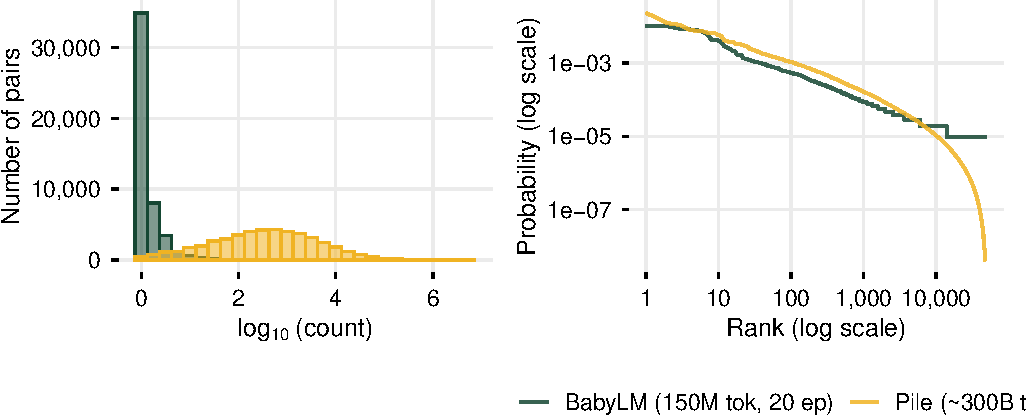
\includegraphics[keepaspectratio]{writeup_files/figure-pdf/fig-corpus-freq-1.pdf}}

}

\caption{\label{fig-corpus-freq}Frequency distributions for the
\textasciitilde47K corpus binomials in the BabyLM training corpus (150M
tokens, 20 epochs) and the Pile. Left: histogram of log\(_{10}\) raw
counts. Right: rank-frequency plot treating counts as a probability
distribution (probability = count / \(\sum\) counts); both axes
log-scaled. BabyLM's distribution is heavily concentrated at a single
occurrence per pair (70.7\% of pairs appear exactly once), whereas Pile
frequencies span several orders of magnitude with a median of 365
occurrences per pair.}

\end{figure}%

The BabyLM training corpus is a 150M-token collection of child-directed
and informal text (CHILDES, BNC Spoken, children's books, OpenSubtitles,
Wikipedia), trained for 20 epochs. The Pile is a
\textasciitilde300B-token web-scraped corpus used to train the Pythia
family. For each of the \textasciitilde47K corpus binomials, we
extracted 3-gram counts (i.e., the frequency of ``word\(_1\) and
word\(_2\)'' and its reverse) from each corpus via infini-gram
\citep{liu2024infinigram}. As Figure~\ref{fig-corpus-freq} shows, the
BabyLM corpus produces a highly degenerate frequency distribution:
70.7\% of binomials appear exactly once, 87.4\% appear at most twice,
and 98.2\% appear at most ten times, with a maximum of 1,095
occurrences. The Pile distribution is far richer: the median binomial
appears 365 times, the 25th percentile is 62 occurrences, and the 99th
percentile exceeds 77,000.

In absolute training exposure terms (accounting for BabyLM's 20 epochs),
the most frequent BabyLM binomials are seen at most
\textasciitilde21,900 times total across all training steps, while the
equivalent Pile binomials are seen over 1.5 million times in a single
pass. Even the median Pile binomial (365 occurrences per pass)
substantially exceeds BabyLM's total exposure for a typical singleton
binomial (1 × 20 = 20 exposures). This gap in absolute exposure is why
the two corpora cannot be placed on a common developmental axis, and why
the frequency range available for the moderation analysis differs so
sharply between them.

\section{Ordering-Source Regression}\label{sec-appendix-relfreq}

Full results for Equation~\ref{eq-relfreq}: the abstract component
\(\hat{y}\) (\texttt{y\_pred}), the corpus's own attested order for that
binomial (\texttt{rel\_freq}), total binomial frequency
(\texttt{log\_freq}), the two moderations, and the residual-scale term.
All four variables are z-scored within each fit, so coefficients are
standardized betas: a one-standard-deviation change in the predictor
moves the model's ordering preference by that many standard deviations.
Standardizing the outcome as well is what makes the coefficients
comparable across models, attention conditions, and training
checkpoints, since the spread of \texttt{y\_true} differs between fits.

46,757 binomials enter the smallest fit and 48,478 the largest.

Two limits on how far the moderation terms should be read.
\texttt{rel\_freq} is estimated from counts, so it is less reliable for
rare binomials, and a less reliable predictor carries an attenuated
coefficient: part of every positive
\texttt{rel\_freq}\(\times\)\texttt{log\_freq} estimate is that
attenuation rather than storage. Admitting singly-attested binomials
trades one form of this problem for another. Nothing is discarded, but a
binomial seen once now sits at the boundary \(\pm 0.5\),
indistinguishable from one seen a thousand times in a single order. The
effect is strongest for BabyLM, where 92\% of items take a boundary
value and the first seven frequency deciles are entirely singletons, and
mild for the large-scale models, where roughly 8\% sit at a boundary and
\texttt{rel\_freq} varies continuously through its range. The two
nevertheless return moderation estimates of the same magnitude, which is
the reassuring outcome: if the coefficient were mostly a record of how
often the predictor saturates, the corpus at 92\% saturation and the
corpora at 8\% would not agree. The comparison between attention
conditions is unaffected in either case, since \texttt{rel\_freq} is the
identical predictor carrying identical noise in both conditions, so
whatever attenuation contributes cancels from the difference. Where a
single number is wanted, the condition contrast is the defensible one.

\begingroup\fontsize{7}{9}\selectfont

\begin{longtable}[t]{llllll}

\toprule
Model & Condition & \texttt{y\_pred} & \texttt{rel\_freq} & \texttt{y\_pred} $\times$ \texttt{log\_freq} & \texttt{rel\_freq} $\times$ \texttt{log\_freq}\\
\midrule
\endfirsthead
\multicolumn{6}{@{}l}{\textit{(continued)}}\\
\toprule
Model & Condition & \texttt{y\_pred} & \texttt{rel\_freq} & \texttt{y\_pred} $\times$ \texttt{log\_freq} & \texttt{rel\_freq} $\times$ \texttt{log\_freq}\\
\midrule
\endhead

\endfoot
\bottomrule
\endlastfoot
 & Full context & 0.418 [0.411, 0.426] & 0.258 [0.251, 0.266] & 0.002 [-0.006, 0.009] & 0.115 [0.107, 0.124]\\
\nopagebreak
\multirow{-2}{*}{\raggedright\arraybackslash BabyLM-125M} & Attention-zeroed & 0.388 [0.380, 0.396] & 0.202 [0.194, 0.210] & -0.015 [-0.022, -0.008] & 0.055 [0.047, 0.063]\\
\cmidrule{1-6}\pagebreak[0]
 & Full context & 0.434 [0.426, 0.442] & 0.221 [0.213, 0.229] & -0.006 [-0.013, 0.001] & 0.104 [0.095, 0.113]\\
\nopagebreak
\multirow{-2}{*}{\raggedright\arraybackslash BabyLM-350M} & Attention-zeroed & 0.370 [0.362, 0.378] & 0.200 [0.192, 0.208] & -0.011 [-0.018, -0.004] & 0.060 [0.052, 0.069]\\
\cmidrule{1-6}\pagebreak[0]
 & Full context & 0.332 [0.324, 0.340] & 0.341 [0.333, 0.348] & 0.001 [-0.006, 0.009] & 0.103 [0.094, 0.111]\\
\nopagebreak
\multirow{-2}{*}{\raggedright\arraybackslash BabyLM-1.3B} & Attention-zeroed & 0.275 [0.267, 0.283] & 0.253 [0.245, 0.262] & -0.014 [-0.021, -0.006] & 0.034 [0.025, 0.043]\\
\cmidrule{1-6}\pagebreak[0]
 & Full context & 0.489 [0.482, 0.497] & 0.291 [0.283, 0.298] & -0.015 [-0.021, -0.008] & 0.139 [0.133, 0.146]\\
\nopagebreak
\multirow{-2}{*}{\raggedright\arraybackslash GPT-2} & Attention-zeroed & 0.683 [0.676, 0.689] & 0.088 [0.082, 0.095] & -0.043 [-0.050, -0.036] & 0.018 [0.013, 0.024]\\
\cmidrule{1-6}\pagebreak[0]
 & Full context & 0.446 [0.439, 0.454] & 0.328 [0.321, 0.336] & -0.014 [-0.021, -0.007] & 0.143 [0.137, 0.150]\\
\nopagebreak
\multirow{-2}{*}{\raggedright\arraybackslash GPT-2-M} & Attention-zeroed & 0.640 [0.633, 0.646] & 0.123 [0.116, 0.129] & -0.028 [-0.035, -0.021] & 0.025 [0.019, 0.031]\\
\cmidrule{1-6}\pagebreak[0]
 & Full context & 0.454 [0.447, 0.462] & 0.330 [0.323, 0.338] & -0.019 [-0.027, -0.012] & 0.138 [0.132, 0.145]\\
\nopagebreak
\multirow{-2}{*}{\raggedright\arraybackslash GPT-2-L} & Attention-zeroed & 0.566 [0.559, 0.573] & 0.143 [0.135, 0.150] & -0.035 [-0.042, -0.028] & 0.030 [0.024, 0.036]\\
\cmidrule{1-6}\pagebreak[0]
 & Full context & 0.447 [0.439, 0.454] & 0.342 [0.334, 0.349] & -0.022 [-0.030, -0.016] & 0.138 [0.132, 0.145]\\
\nopagebreak
\multirow{-2}{*}{\raggedright\arraybackslash GPT-2-XL} & Attention-zeroed & 0.605 [0.598, 0.612] & 0.131 [0.124, 0.138] & -0.035 [-0.042, -0.028] & 0.034 [0.028, 0.040]\\
\cmidrule{1-6}\pagebreak[0]
 & Full context & 0.462 [0.454, 0.469] & 0.304 [0.296, 0.311] & -0.008 [-0.015, -0.001] & 0.129 [0.122, 0.135]\\
\nopagebreak
\multirow{-2}{*}{\raggedright\arraybackslash Pythia-160M} & Attention-zeroed & 0.506 [0.499, 0.514] & 0.160 [0.152, 0.168] & -0.021 [-0.028, -0.013] & 0.023 [0.017, 0.030]\\
\cmidrule{1-6}\pagebreak[0]
 & Full context & 0.453 [0.445, 0.460] & 0.336 [0.328, 0.344] & -0.026 [-0.033, -0.019] & 0.132 [0.126, 0.139]\\
\nopagebreak
\multirow{-2}{*}{\raggedright\arraybackslash Pythia-410M} & Attention-zeroed & 0.517 [0.510, 0.525] & 0.166 [0.159, 0.173] & -0.038 [-0.045, -0.031] & 0.037 [0.031, 0.043]\\
\cmidrule{1-6}\pagebreak[0]
 & Full context & 0.493 [0.485, 0.500] & 0.323 [0.316, 0.331] & -0.027 [-0.034, -0.021] & 0.117 [0.110, 0.123]\\
\nopagebreak
\multirow{-2}{*}{\raggedright\arraybackslash Pythia-1B} & Attention-zeroed & 0.575 [0.568, 0.582] & 0.150 [0.143, 0.157] & -0.035 [-0.043, -0.028] & 0.033 [0.027, 0.039]\\
\cmidrule{1-6}\pagebreak[0]
 & Full context & 0.534 [0.527, 0.541] & 0.302 [0.295, 0.309] & -0.027 [-0.033, -0.020] & 0.113 [0.107, 0.119]\\
\nopagebreak
\multirow{-2}{*}{\raggedright\arraybackslash OLMo-1B} & Attention-zeroed & 0.592 [0.585, 0.599] & 0.158 [0.151, 0.166] & -0.029 [-0.036, -0.022] & 0.034 [0.028, 0.040]\\
\cmidrule{1-6}\pagebreak[0]
 & Full context & 0.582 [0.575, 0.589] & 0.283 [0.277, 0.290] & -0.022 [-0.028, -0.016] & 0.097 [0.091, 0.102]\\
\nopagebreak
\multirow{-2}{*}{\raggedright\arraybackslash OLMo-7B} & Attention-zeroed & 0.636 [0.630, 0.643] & 0.160 [0.153, 0.167] & -0.028 [-0.035, -0.021] & 0.039 [0.033, 0.044]\\
\cmidrule{1-6}\pagebreak[0]
 & Full context & 0.519 [0.512, 0.526] & 0.303 [0.296, 0.311] & -0.029 [-0.036, -0.023] & 0.099 [0.093, 0.105]\\
\nopagebreak
\multirow{-2}{*}{\raggedright\arraybackslash OLMo-2-1B} & Attention-zeroed & 0.592 [0.585, 0.599] & 0.156 [0.149, 0.163] & -0.037 [-0.044, -0.029] & 0.031 [0.024, 0.037]\\
\cmidrule{1-6}\pagebreak[0]
 & Full context & 0.628 [0.621, 0.634] & 0.238 [0.231, 0.244] & -0.034 [-0.040, -0.027] & 0.068 [0.063, 0.074]\\
\nopagebreak
\multirow{-2}{*}{\raggedright\arraybackslash OLMo-2-7B} & Attention-zeroed & 0.669 [0.663, 0.676] & 0.144 [0.137, 0.150] & -0.033 [-0.039, -0.027] & 0.032 [0.027, 0.038]\\
\cmidrule{1-6}\pagebreak[0]
 & Full context & 0.496 [0.489, 0.503] & 0.323 [0.316, 0.331] & -0.025 [-0.032, -0.018] & 0.116 [0.110, 0.122]\\
\nopagebreak
\multirow{-2}{*}{\raggedright\arraybackslash Llama-1.3B} & Attention-zeroed & 0.560 [0.552, 0.567] & 0.169 [0.162, 0.177] & -0.041 [-0.049, -0.034] & 0.041 [0.035, 0.048]\\
\cmidrule{1-6}\pagebreak[0]
 & Full context & 0.607 [0.601, 0.614] & 0.259 [0.252, 0.265] & -0.037 [-0.043, -0.031] & 0.087 [0.082, 0.093]\\
\nopagebreak
\multirow{-2}{*}{\raggedright\arraybackslash Llama-3-8B} & Attention-zeroed & 0.640 [0.633, 0.647] & 0.143 [0.136, 0.150] & -0.038 [-0.045, -0.032] & 0.037 [0.031, 0.042]\\*


\caption{\label{tbl-relfreq}Ordering-source regression
(Equation~\ref{eq-relfreq}) for all 16 models at their final checkpoint,
by attention condition. All four variables are z-scored within each fit,
so these are standardized betas, comparable across models and
conditions. 95\% credible intervals in brackets. Holistic storage
predicts a negative \texttt{y\_pred} \(\times\) \texttt{log\_freq} and a
positive \texttt{rel\_freq} \(\times\) \texttt{log\_freq}, both
attenuating under attention-zeroing.}

\tabularnewline
\end{longtable}

\endgroup{}

Figure~\ref{fig-relfreq-coefs} shows the two moderation terms across
models and conditions. The pattern is uniform across all sixteen:
\texttt{rel\_freq}\(\times\)\texttt{log\_freq} is credibly positive in
every model under full context and much smaller under attention-zeroing,
while \texttt{y\_pred}\(\times\)\texttt{log\_freq} is credibly negative
in every large-scale model under both conditions. The BabyLM models
match the large-scale ones on the first term and sit nearer zero on the
second, which is what the restricted frequency range would predict:
\texttt{y\_pred}\(\times\)\texttt{log\_freq} is the term that needs
exposure to vary over orders of magnitude before it can be estimated
apart from the main effect.

\begin{figure*}[t]

\centering{

\pandocbounded{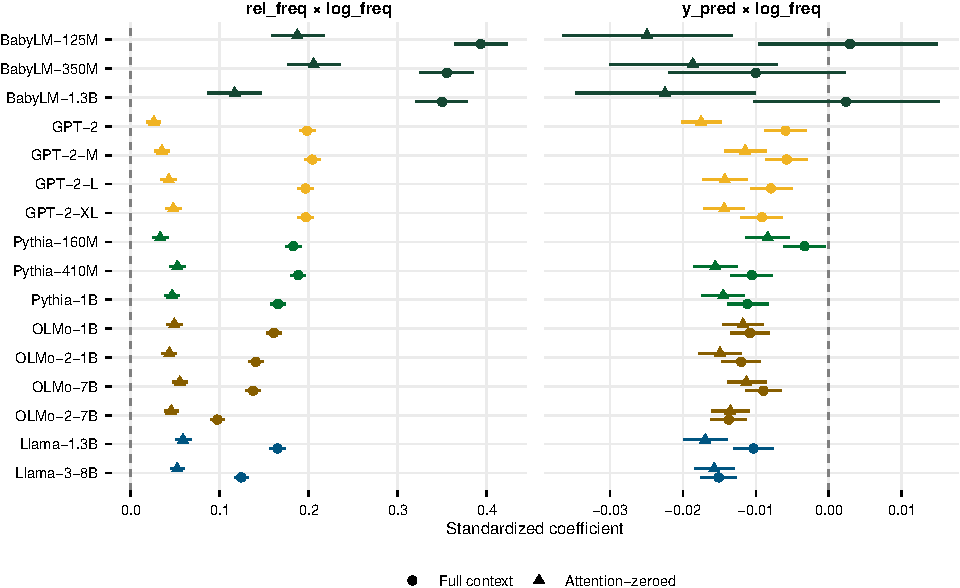
\includegraphics[keepaspectratio]{writeup_files/figure-pdf/fig-relfreq-coefs-1.pdf}}

}

\caption{\label{fig-relfreq-coefs}Moderation terms of
Equation~\ref{eq-relfreq} by model and attention condition. Circles =
full context; triangles = attention-zeroed. Points = posterior mean;
bars = 95\% credible intervals. Left: the corpus's attested order
matters more for frequent binomials, and attention-zeroing removes most
of that. Right: the abstract component matters less for frequent
binomials, and attention-zeroing does not remove it.}

\end{figure*}%

\end{document}
